\begin{figure*}[htbp]
    \centering

    % 第一行左侧的竖排标签
    \begin{minipage}{0.09\textwidth}
        \centering
        Full
        Fine-tuning
    \end{minipage}
    \hfill
    % 第一行图片
    \begin{minipage}{0.22\textwidth}
        \centering
        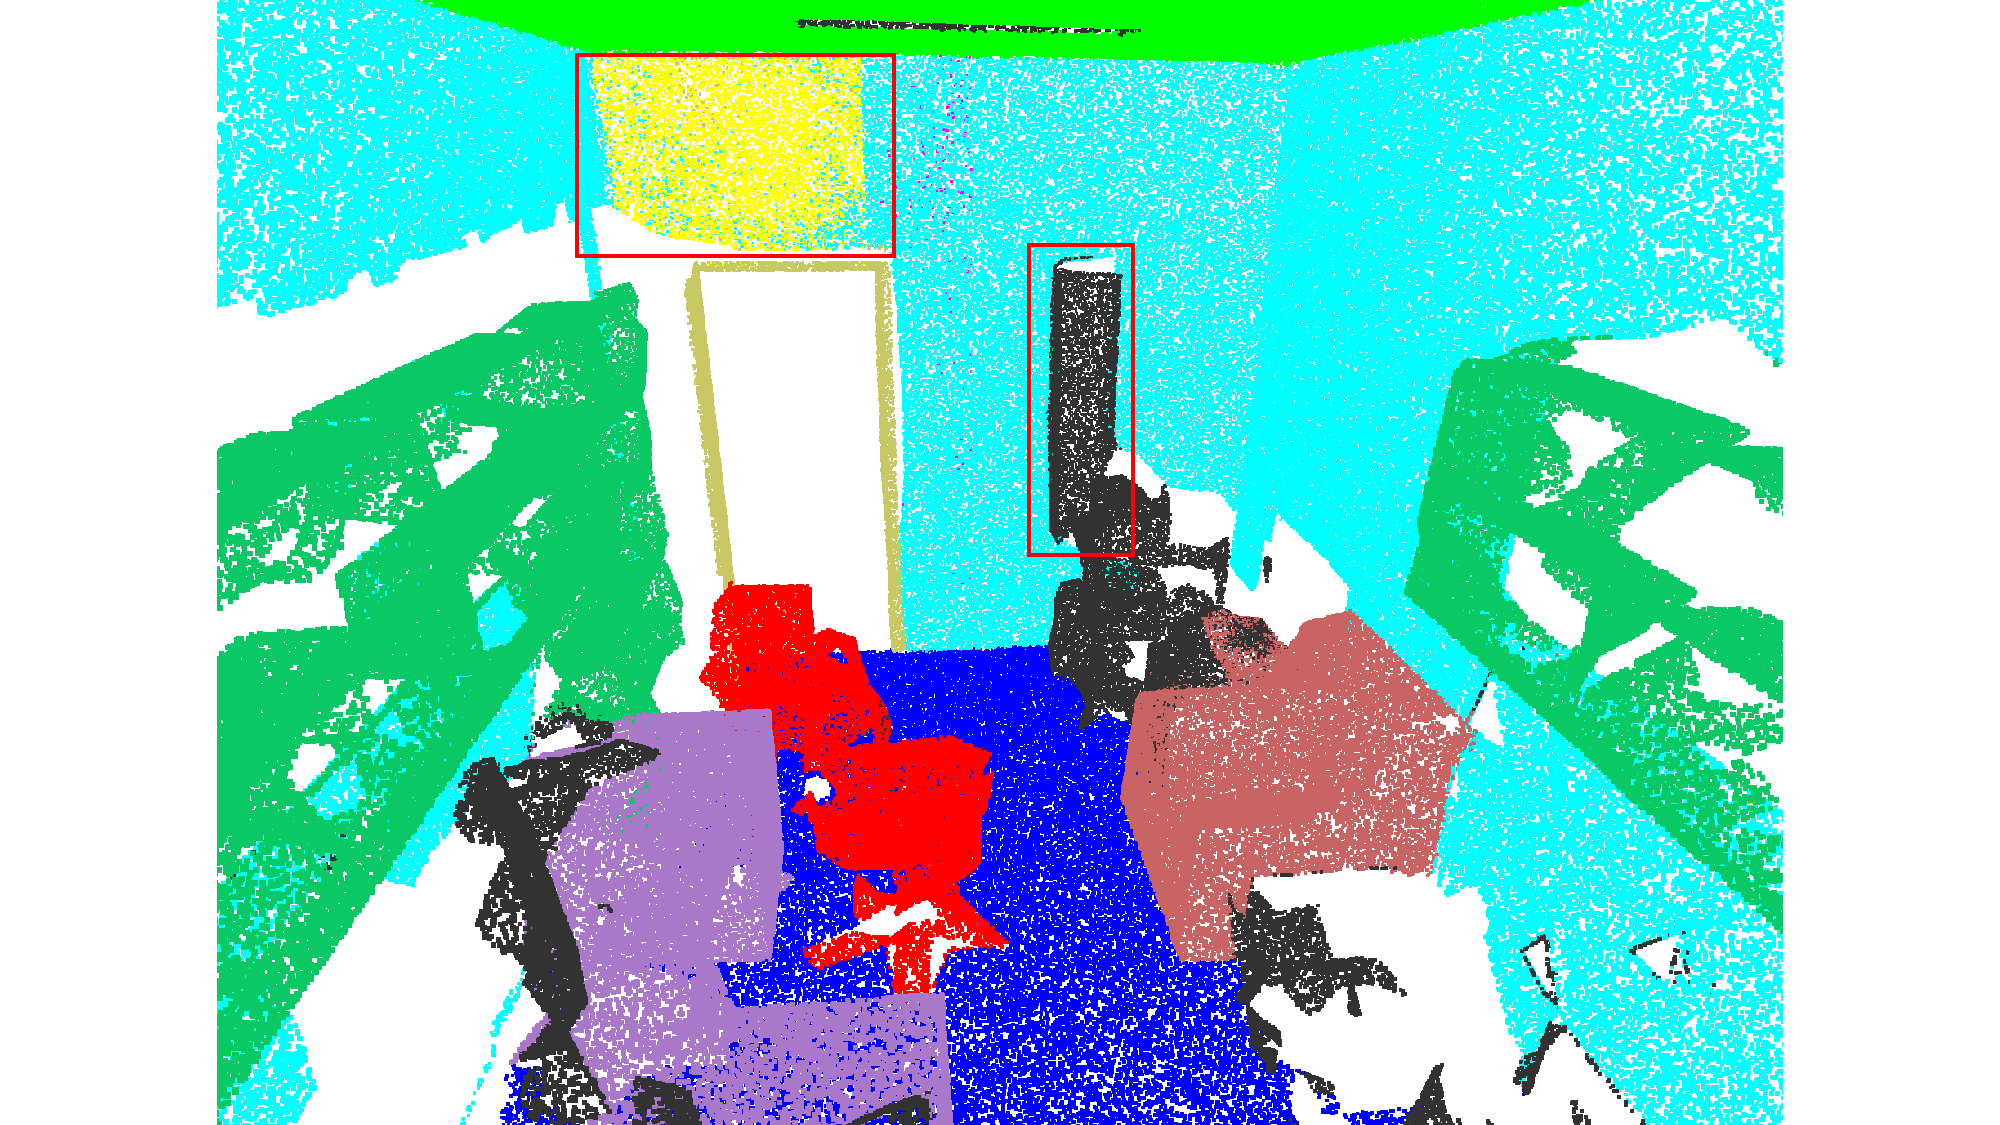
\includegraphics[width=\textwidth]{fig/supplement/semantic_segmentation/office_9/PT_office_9.pdf}
    \end{minipage}
    \hfill
    \begin{minipage}{0.22\textwidth}
        \centering
        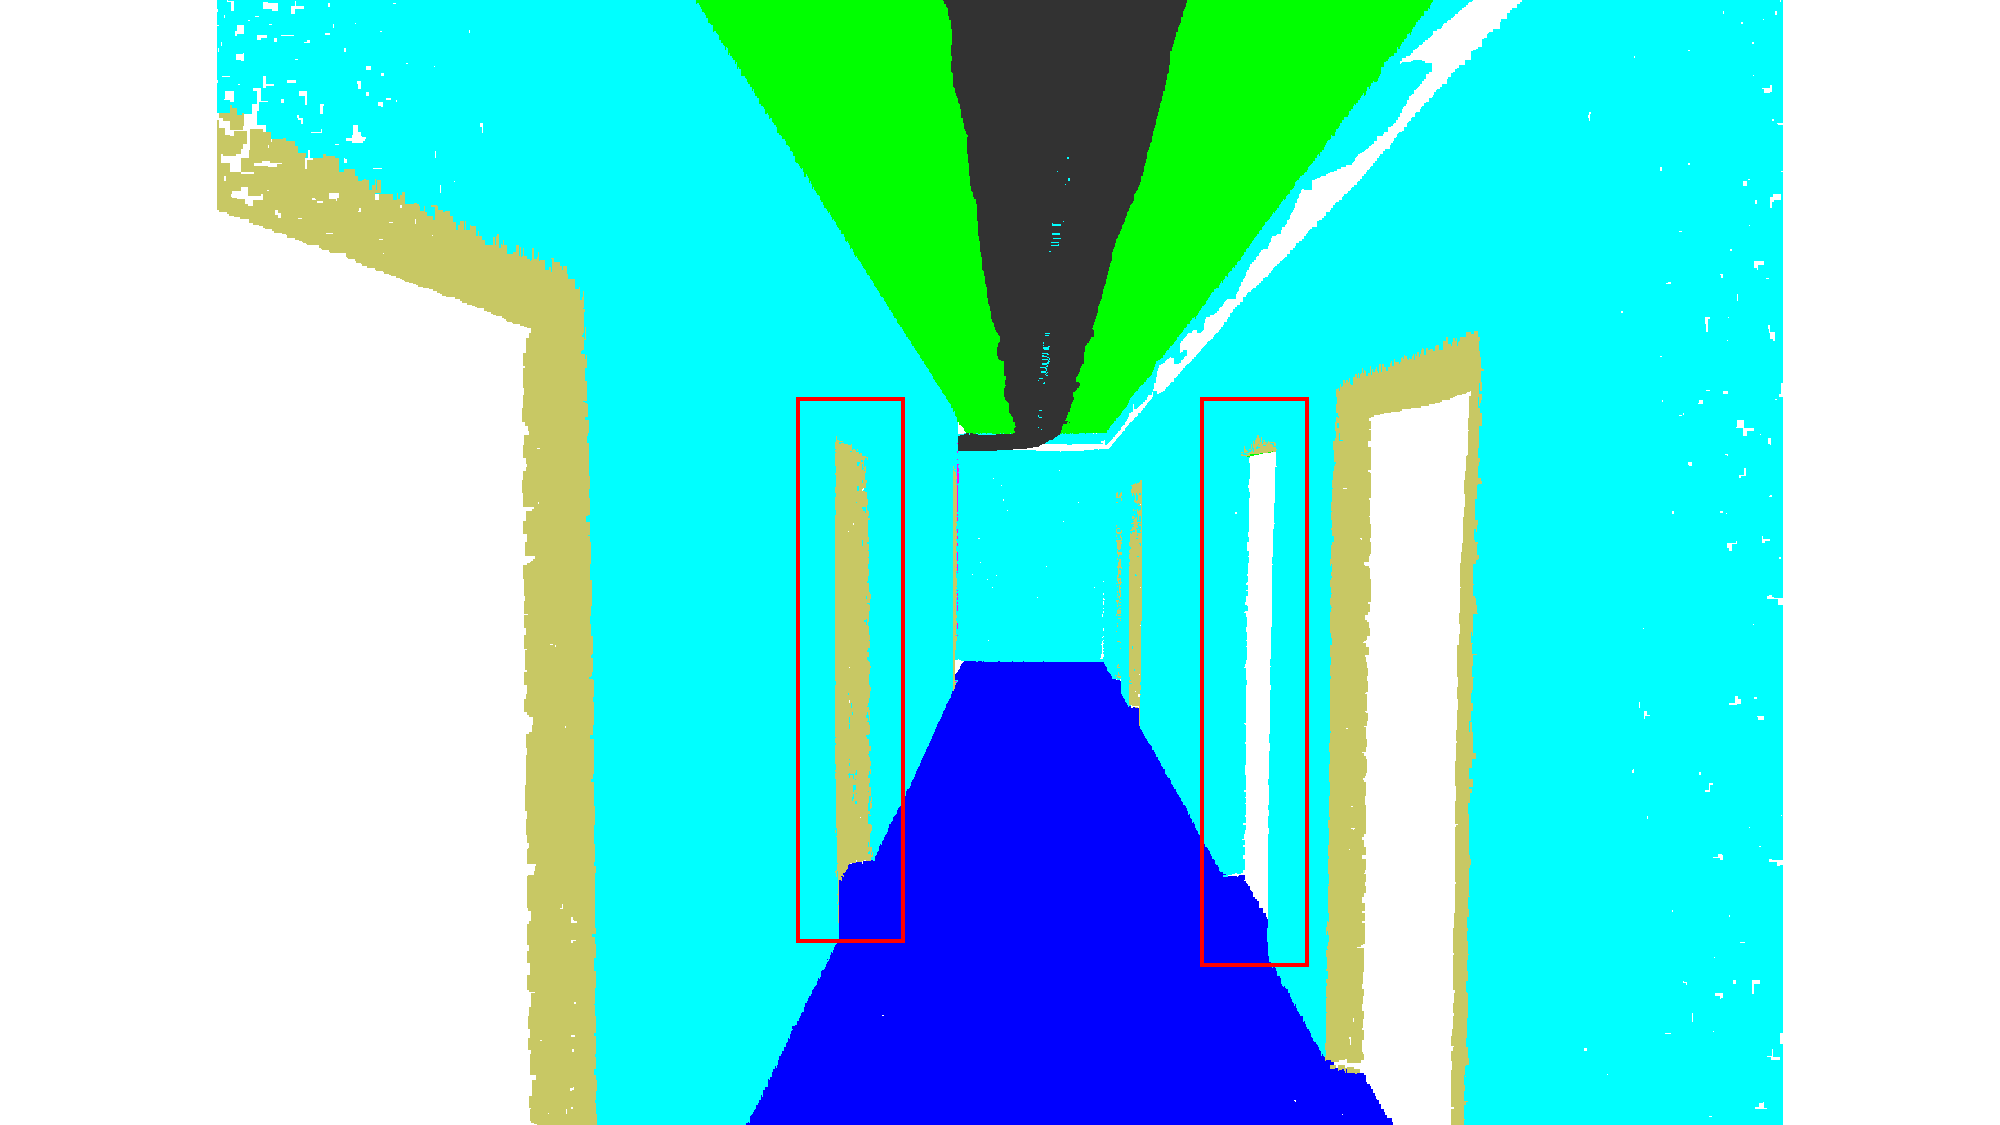
\includegraphics[width=\textwidth]{fig/supplement/semantic_segmentation/hallway_10/PT_hallway_10.pdf} % 替换为你的图片路径
    \end{minipage}
    \hfill
    \begin{minipage}{0.22\textwidth}
        \centering
        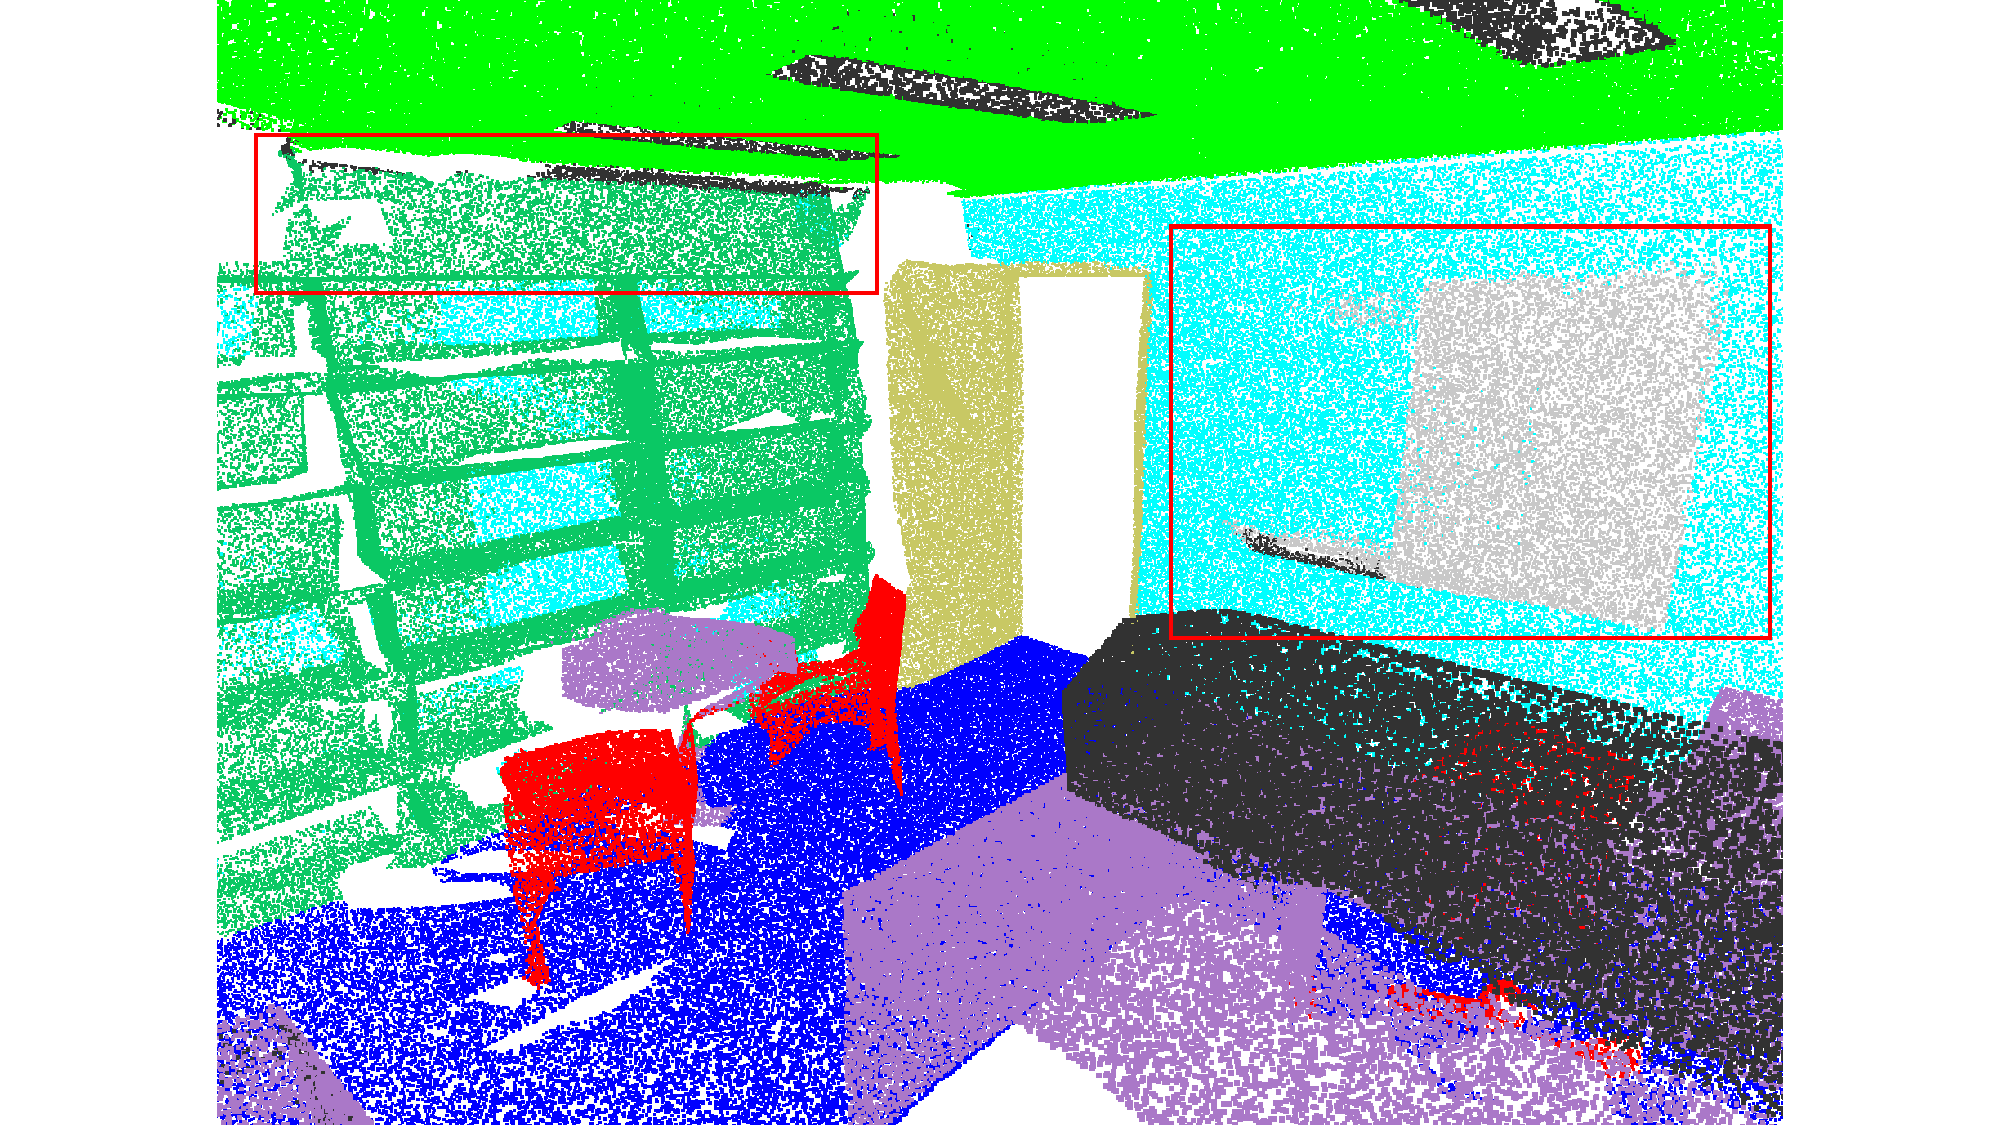
\includegraphics[width=\textwidth]{fig/supplement/semantic_segmentation/office_35/PT_office_35.pdf}
    \end{minipage}
    \hfill
    \begin{minipage}{0.22\textwidth}
        \centering
        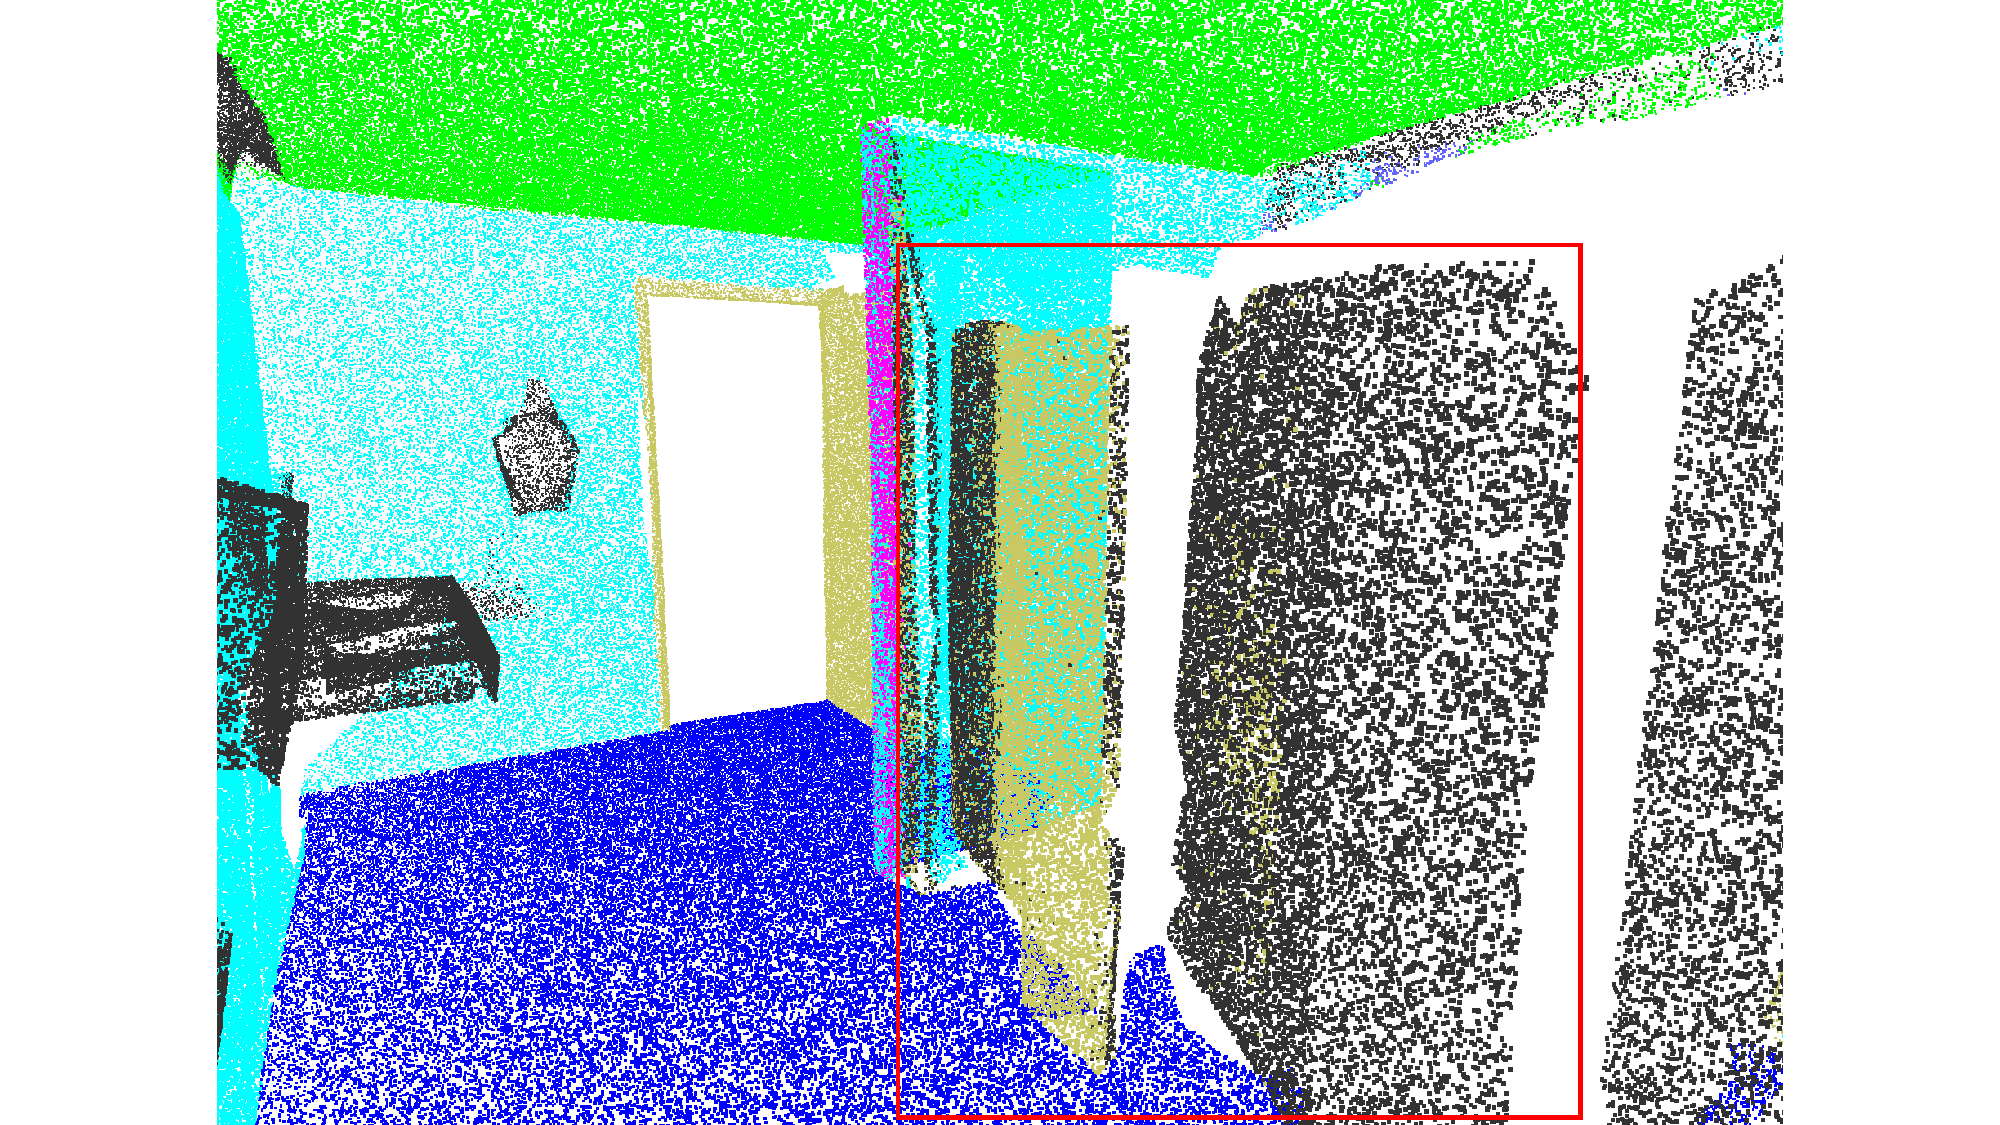
\includegraphics[width=\textwidth]{fig/supplement/semantic_segmentation/wc_2/PT_wc_2.pdf}
    \end{minipage}
    \hfill

    % 换行
    \vspace{0.5em}

    % 第二行左侧的竖排标签
    \begin{minipage}{0.09\textwidth}
        \centering
        DAPT
    \end{minipage}
    \hfill
    % 第二行图片
    \begin{minipage}{0.22\textwidth}
        \centering
        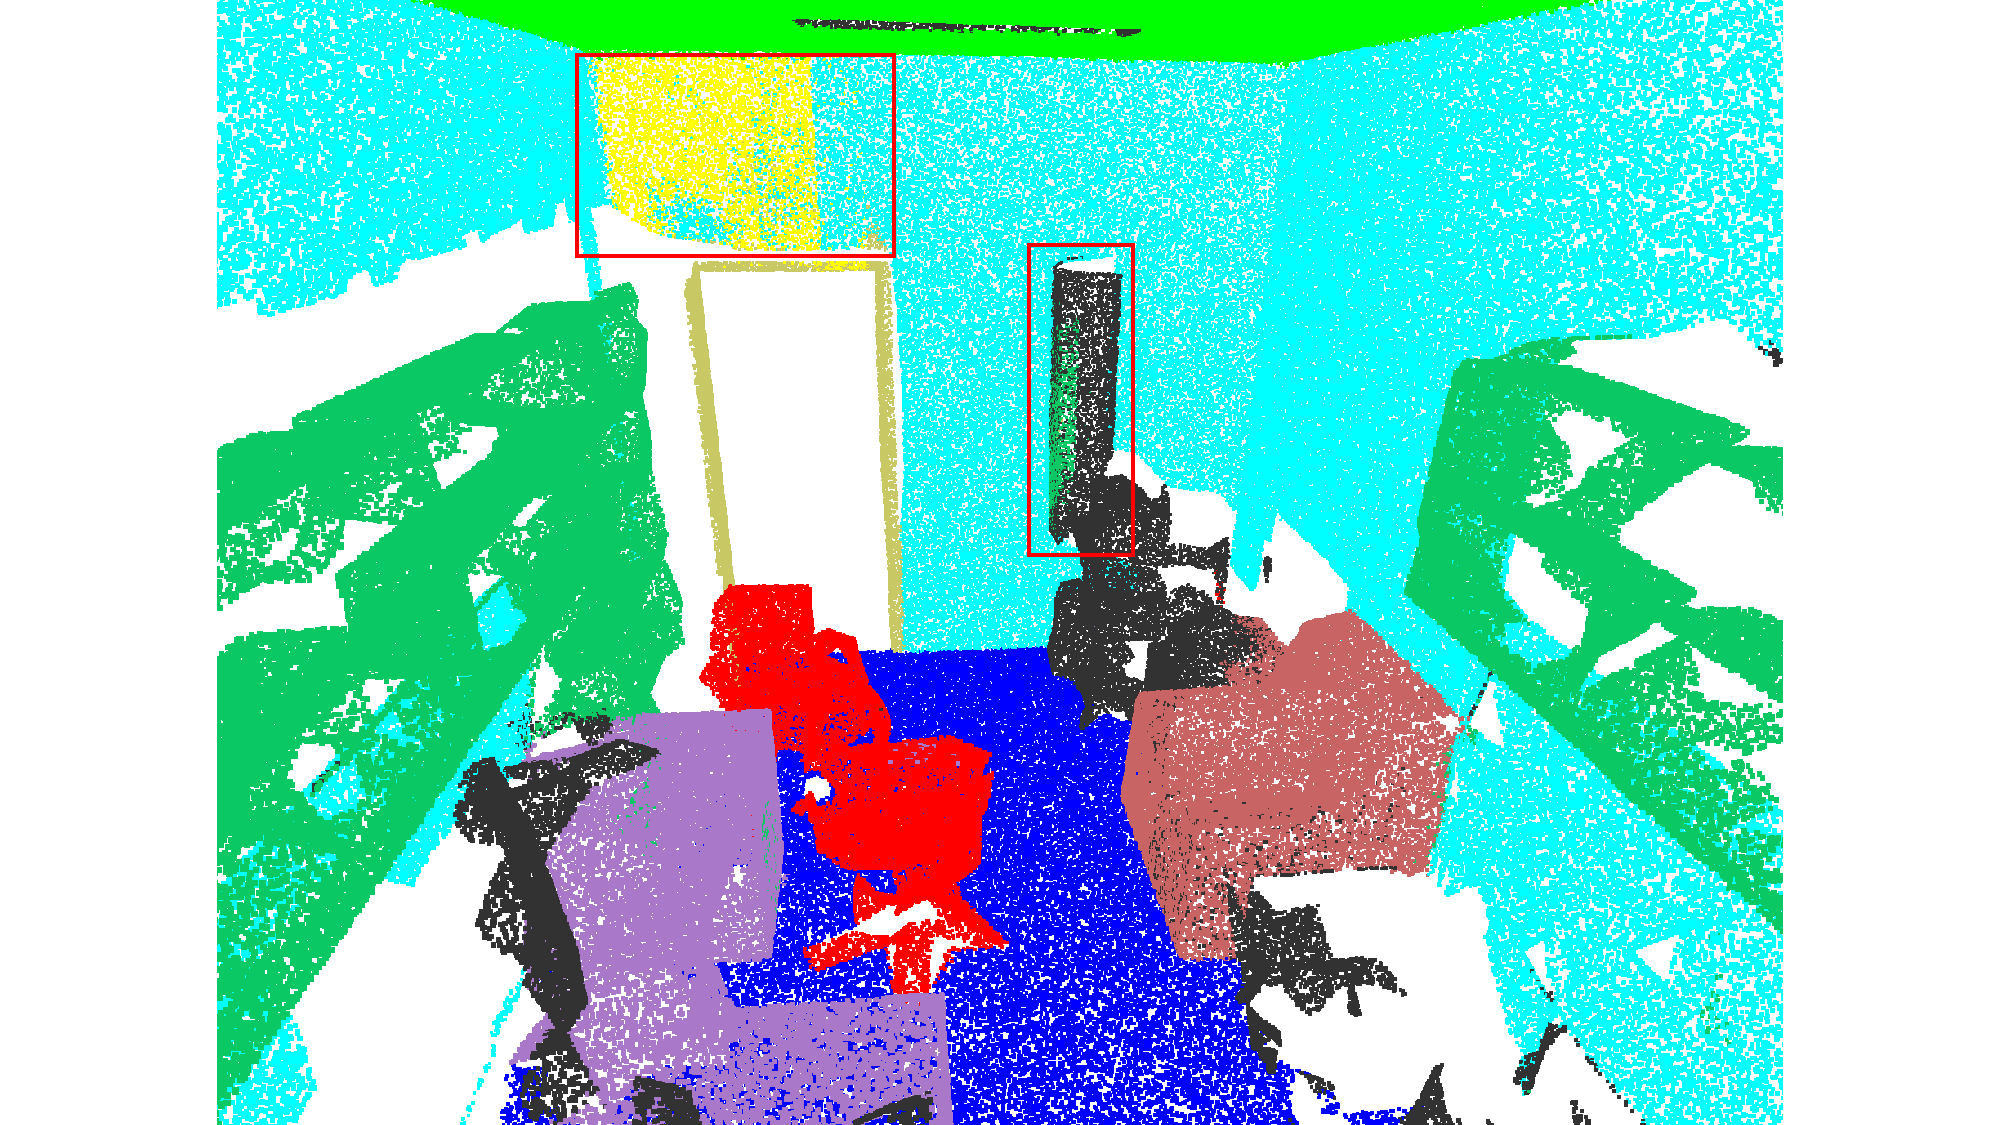
\includegraphics[width=\textwidth]{fig/supplement/semantic_segmentation/office_9/DAPT_office_9.pdf}
    \end{minipage}
    \hfill
    \begin{minipage}{0.22\textwidth}
        \centering
        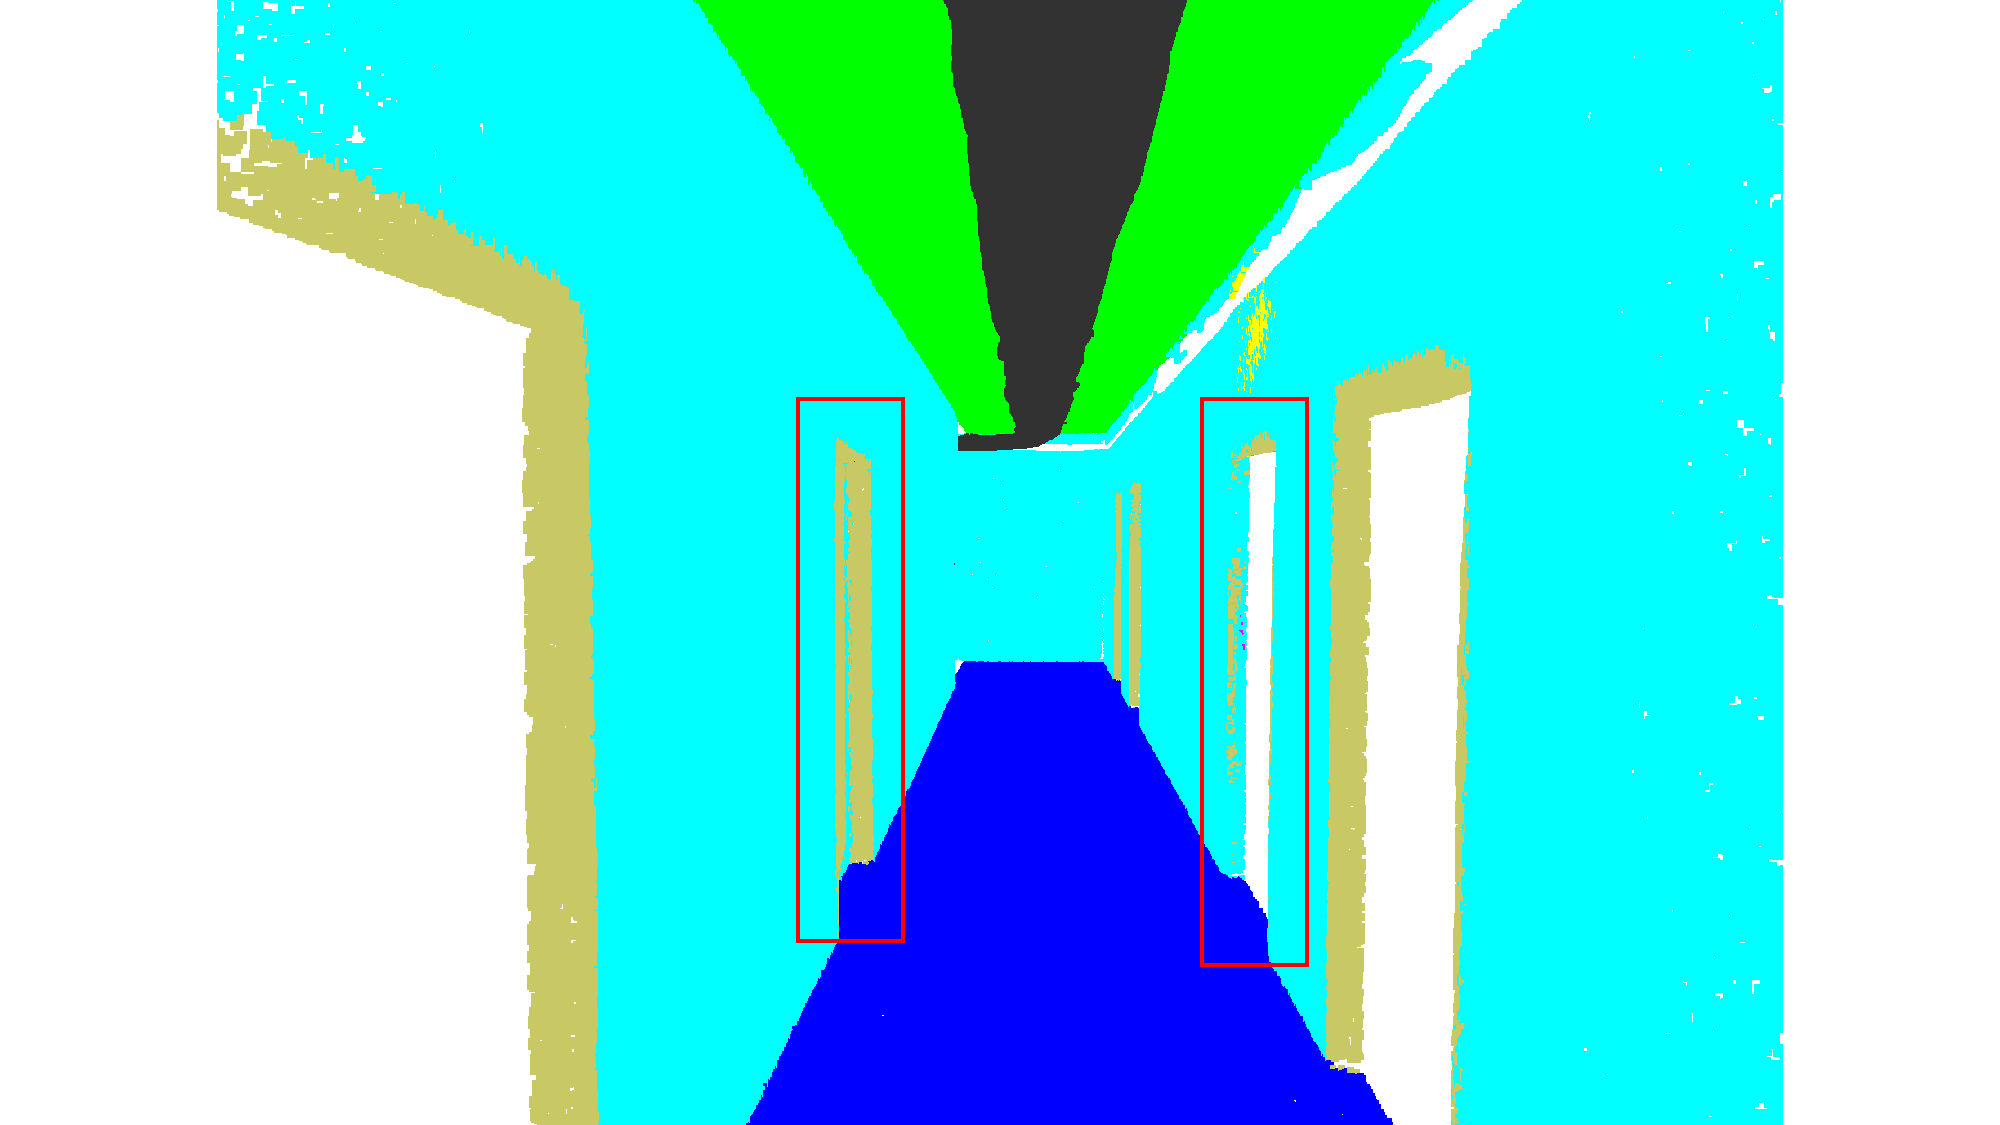
\includegraphics[width=\textwidth]{fig/supplement/semantic_segmentation/hallway_10/DAPT_hallway_10.pdf}
    \end{minipage}
    \hfill
    \begin{minipage}{0.22\textwidth}
        \centering
        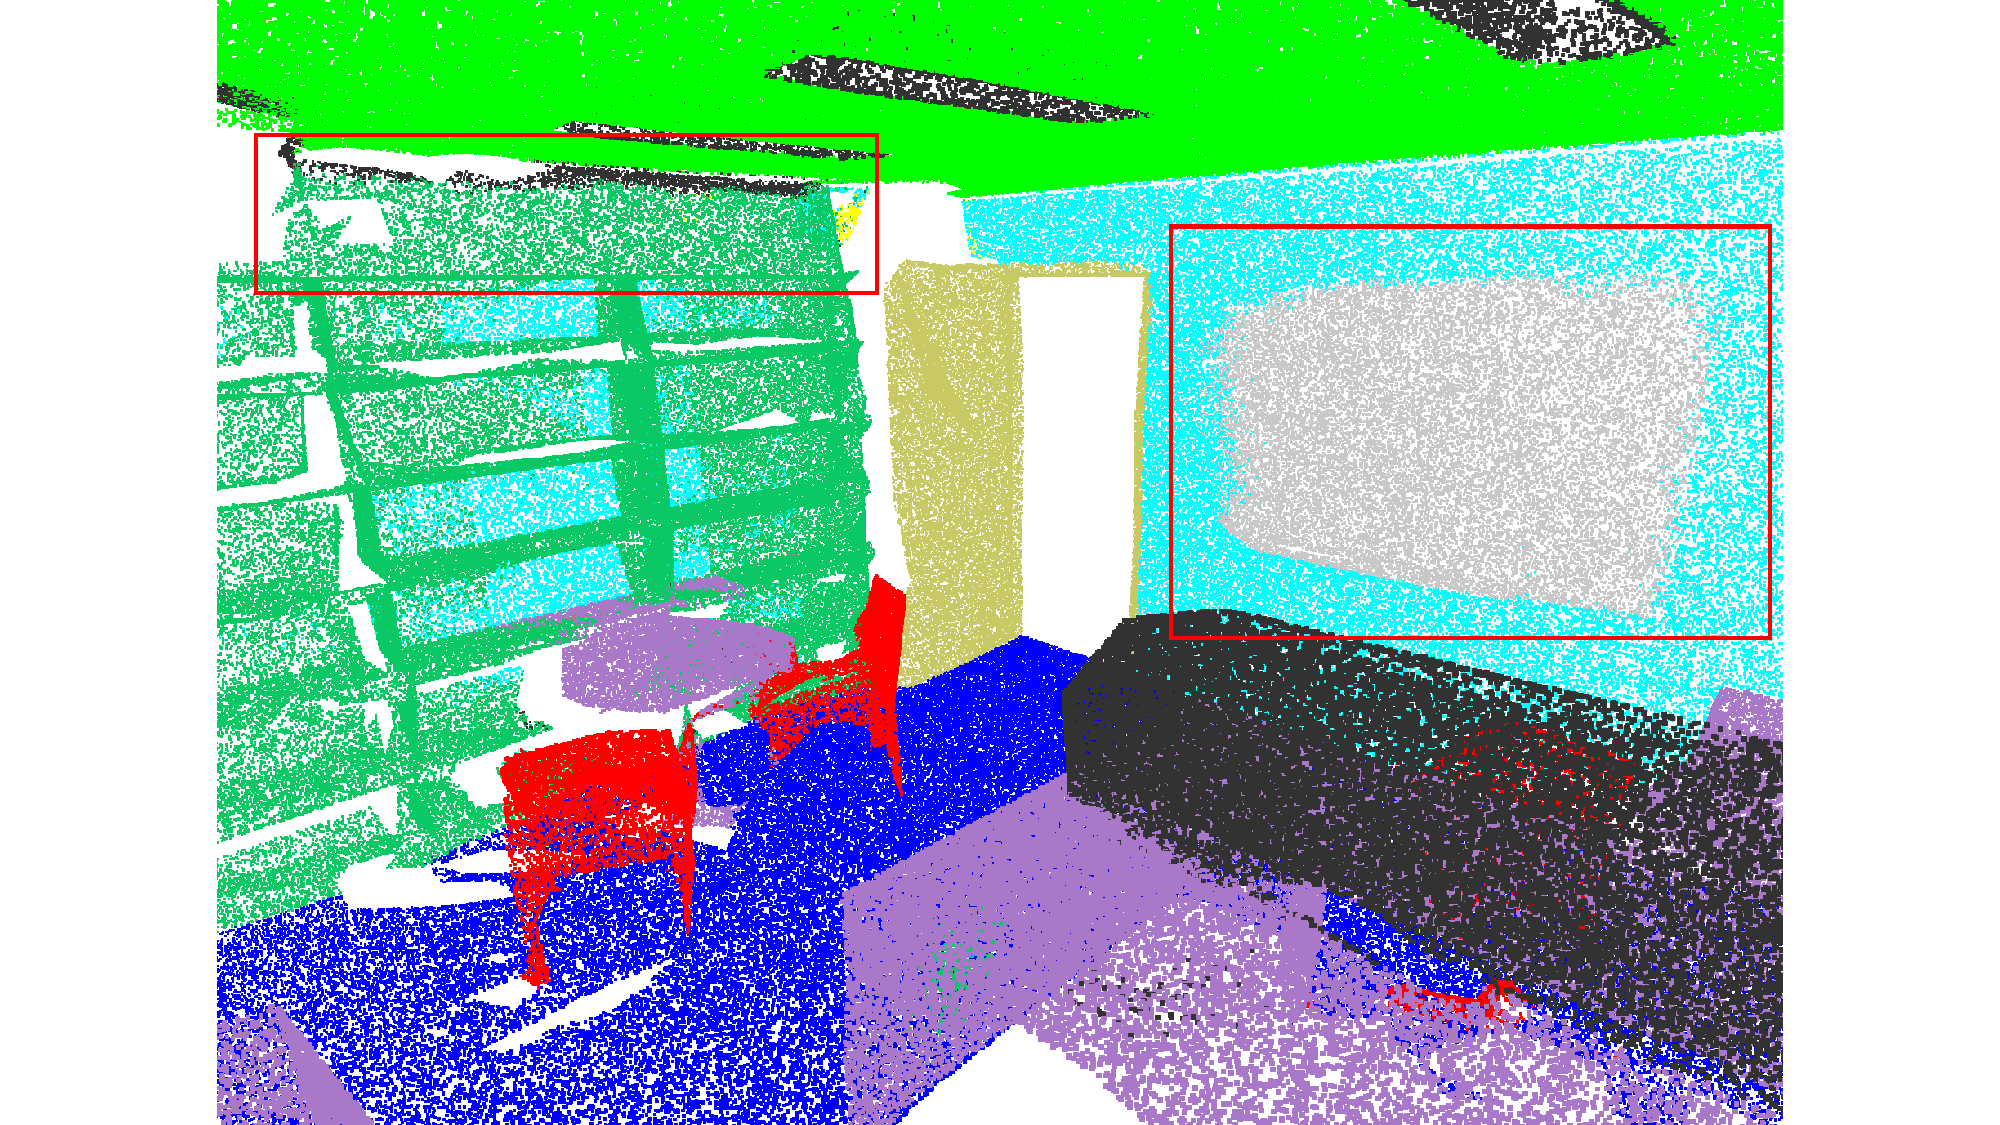
\includegraphics[width=\textwidth]{fig/supplement/semantic_segmentation/office_35/DAPT_office_35.pdf}
    \end{minipage}
    \hfill
    \begin{minipage}{0.22\textwidth}
        \centering
        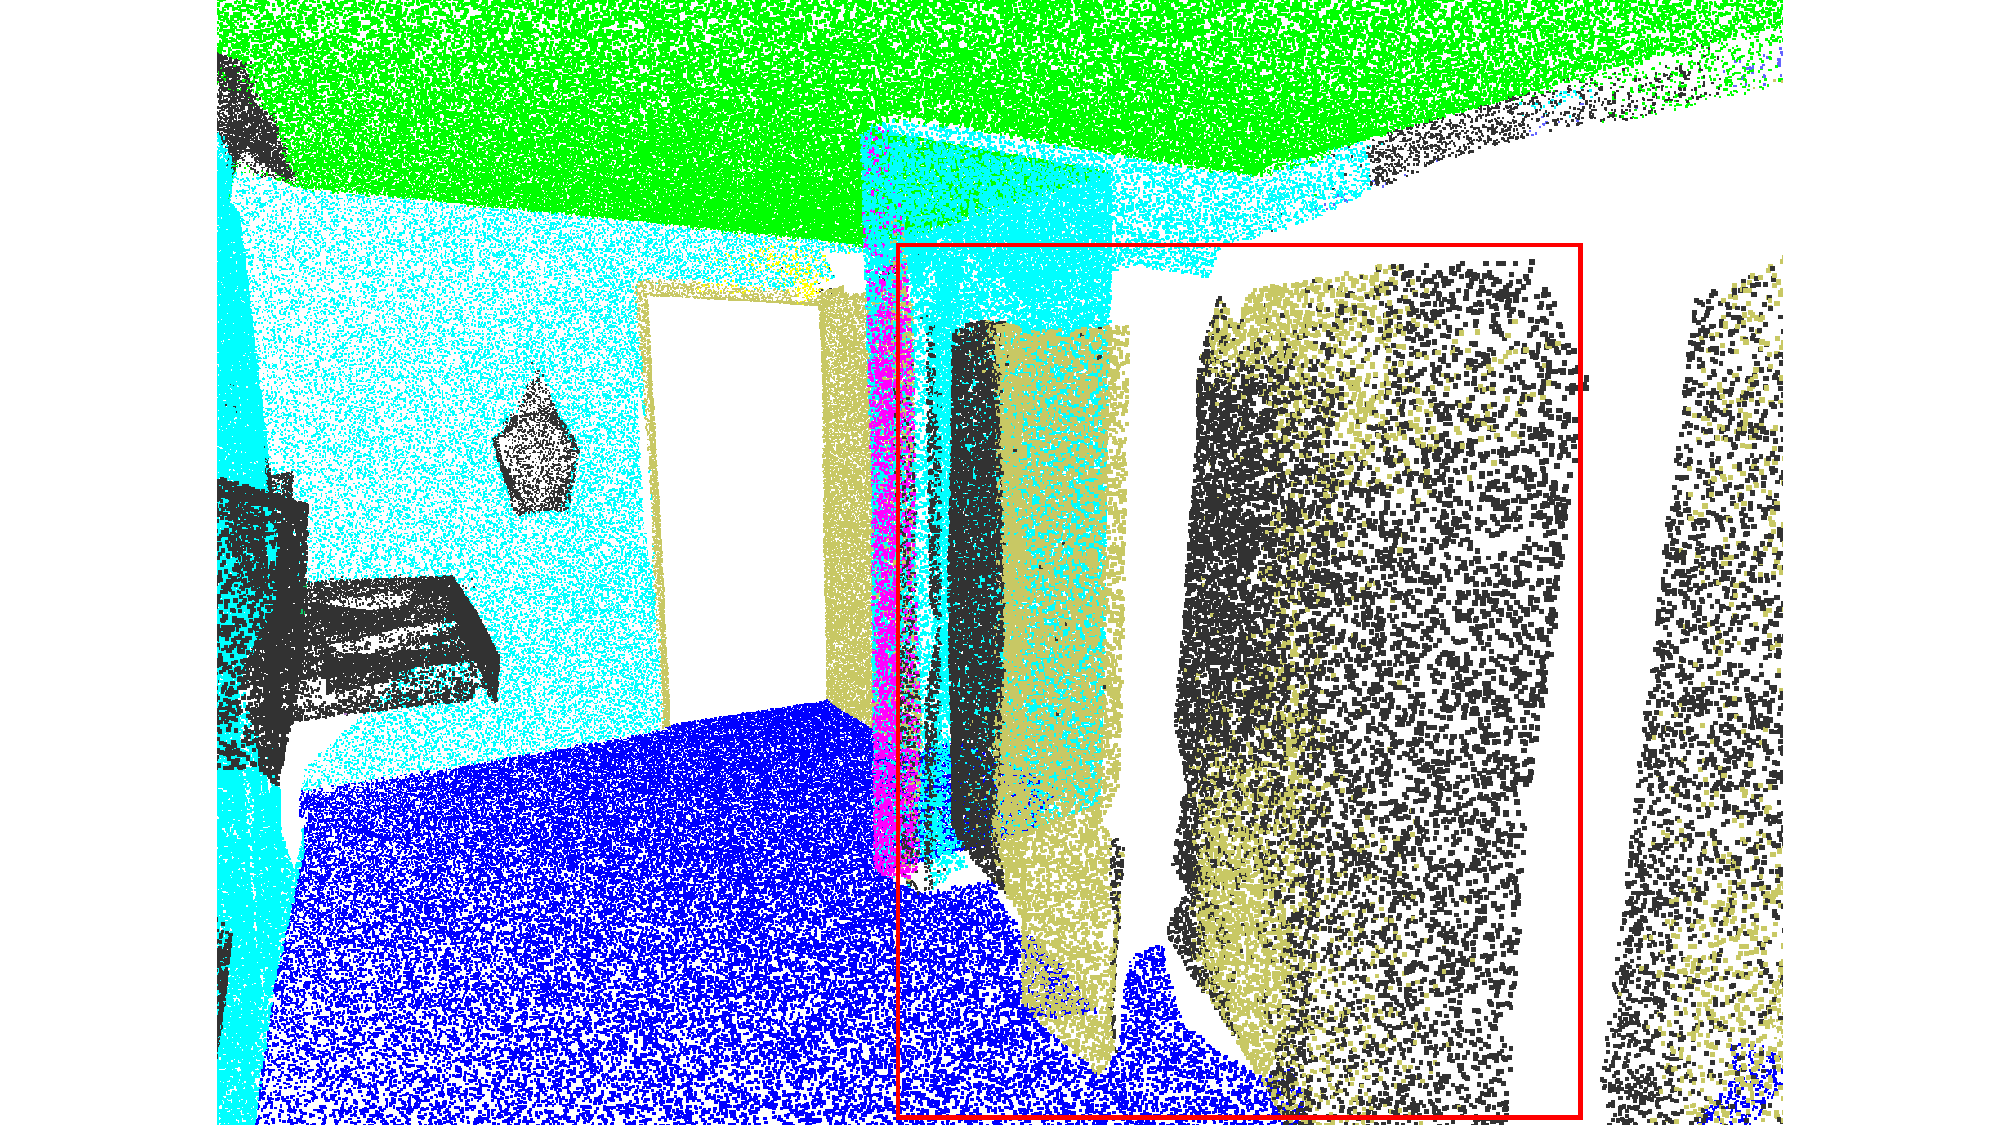
\includegraphics[width=\textwidth]{fig/supplement/semantic_segmentation/wc_2/DAPT_wc_2.pdf}
    \end{minipage}
    \hfill

    % 换行
    \vspace{0.5em}

    % 第三行左侧的竖排标签
    \begin{minipage}{0.09\textwidth}
        \centering
        IDPT
    \end{minipage}
    \hfill
    % 第三行图片
    \begin{minipage}{0.22\textwidth}
        \centering
        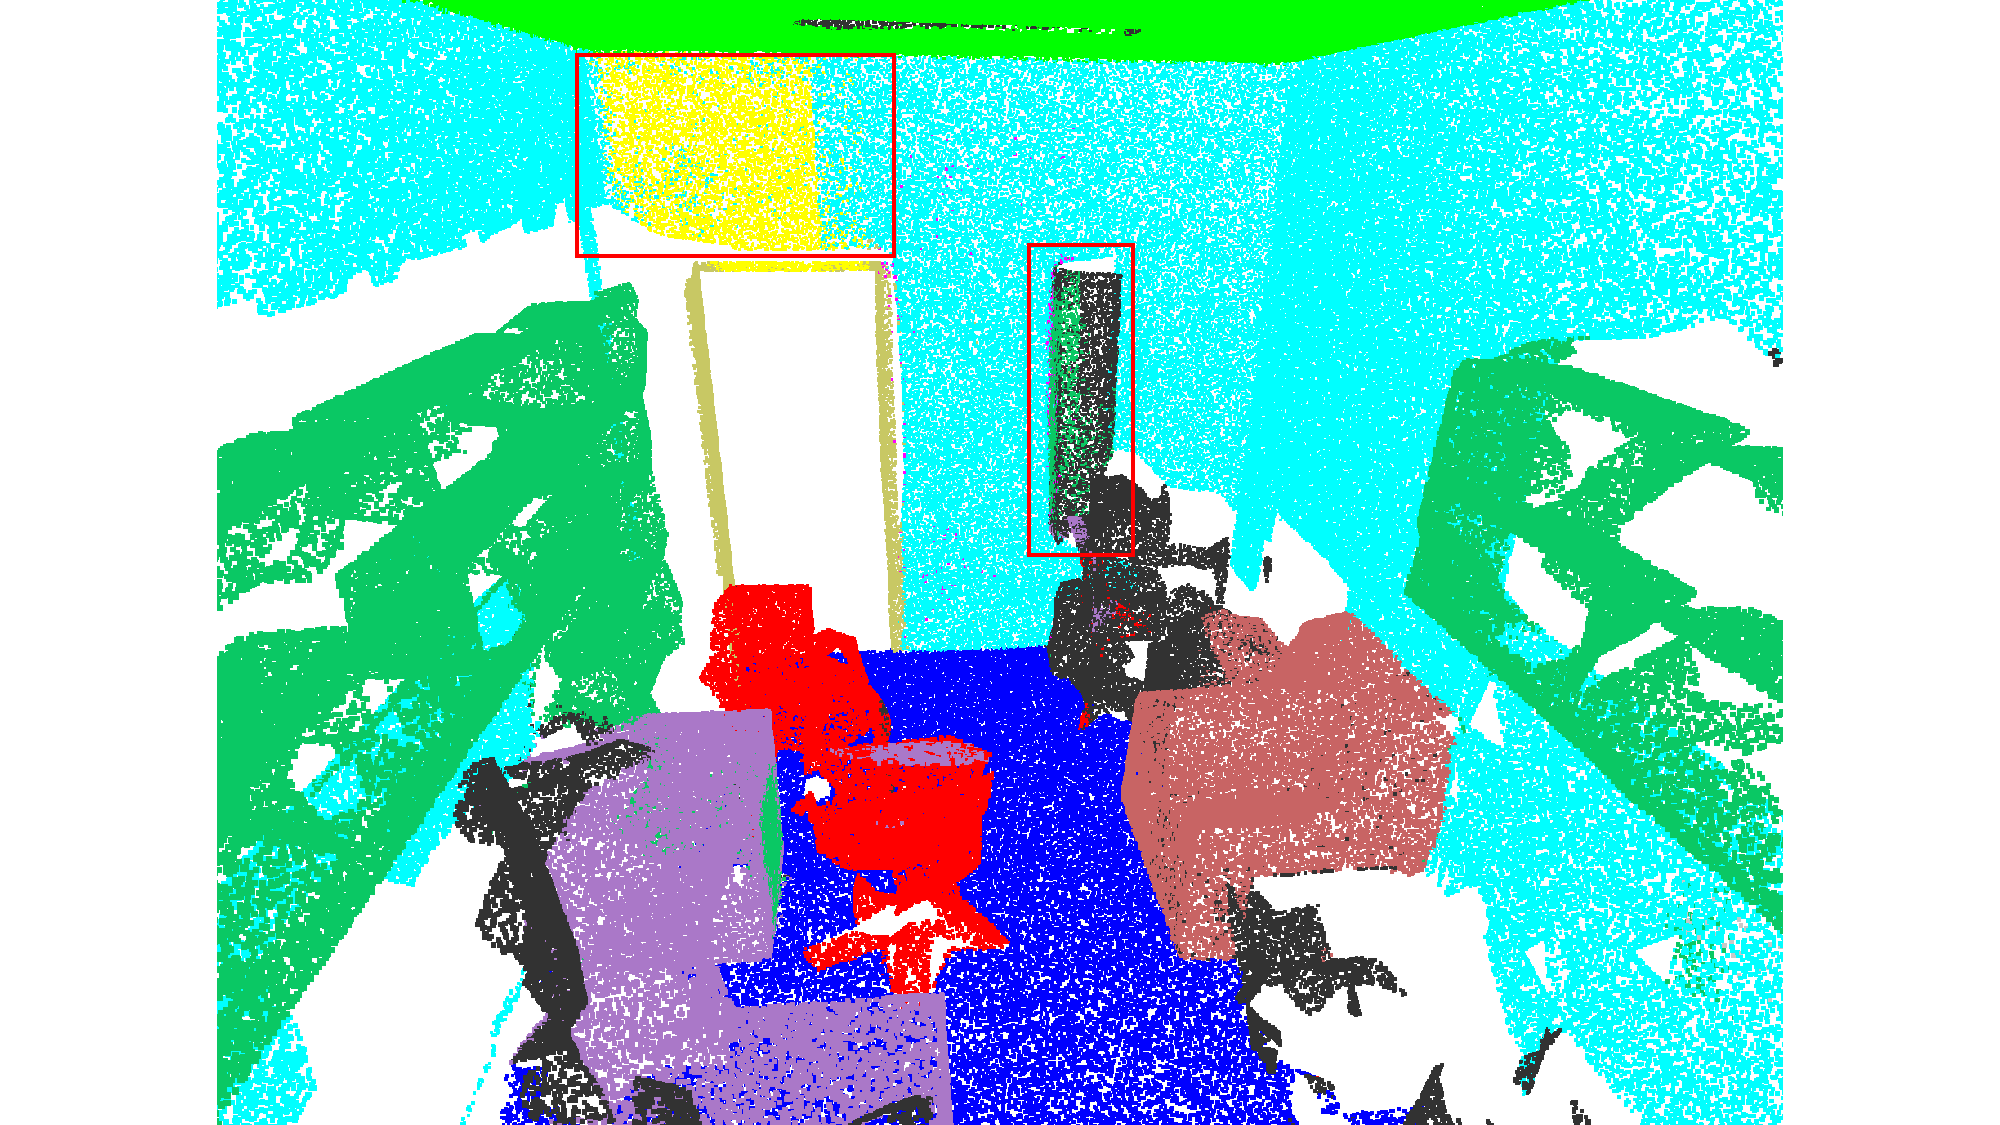
\includegraphics[width=\textwidth]{fig/supplement/semantic_segmentation/office_9/IDPT_office_9.pdf}
    \end{minipage}
    \hfill
    \begin{minipage}{0.22\textwidth}
        \centering
        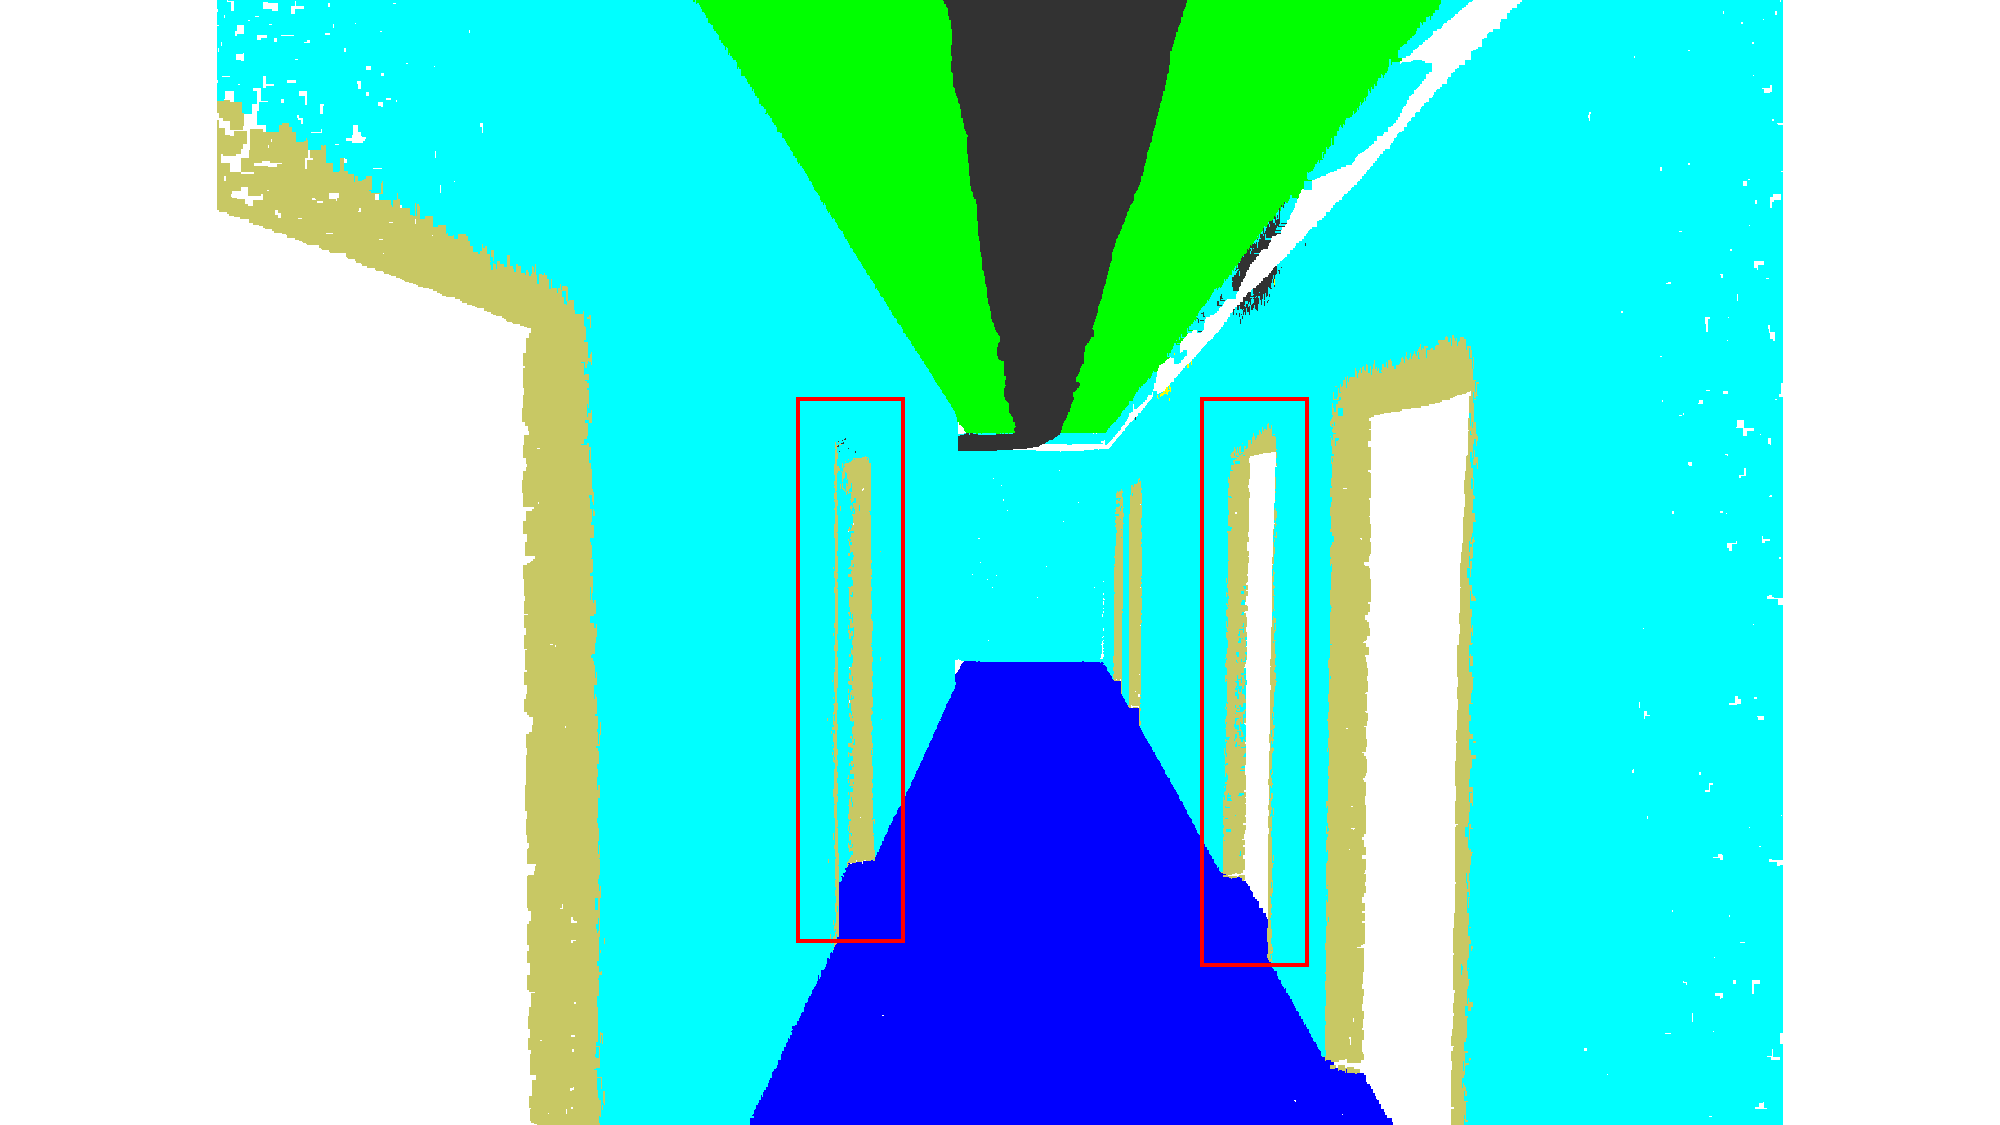
\includegraphics[width=\textwidth]{fig/supplement/semantic_segmentation/hallway_10/IDPT_hallway_10.pdf}
    \end{minipage}
    \hfill
    \begin{minipage}{0.22\textwidth}
        \centering
        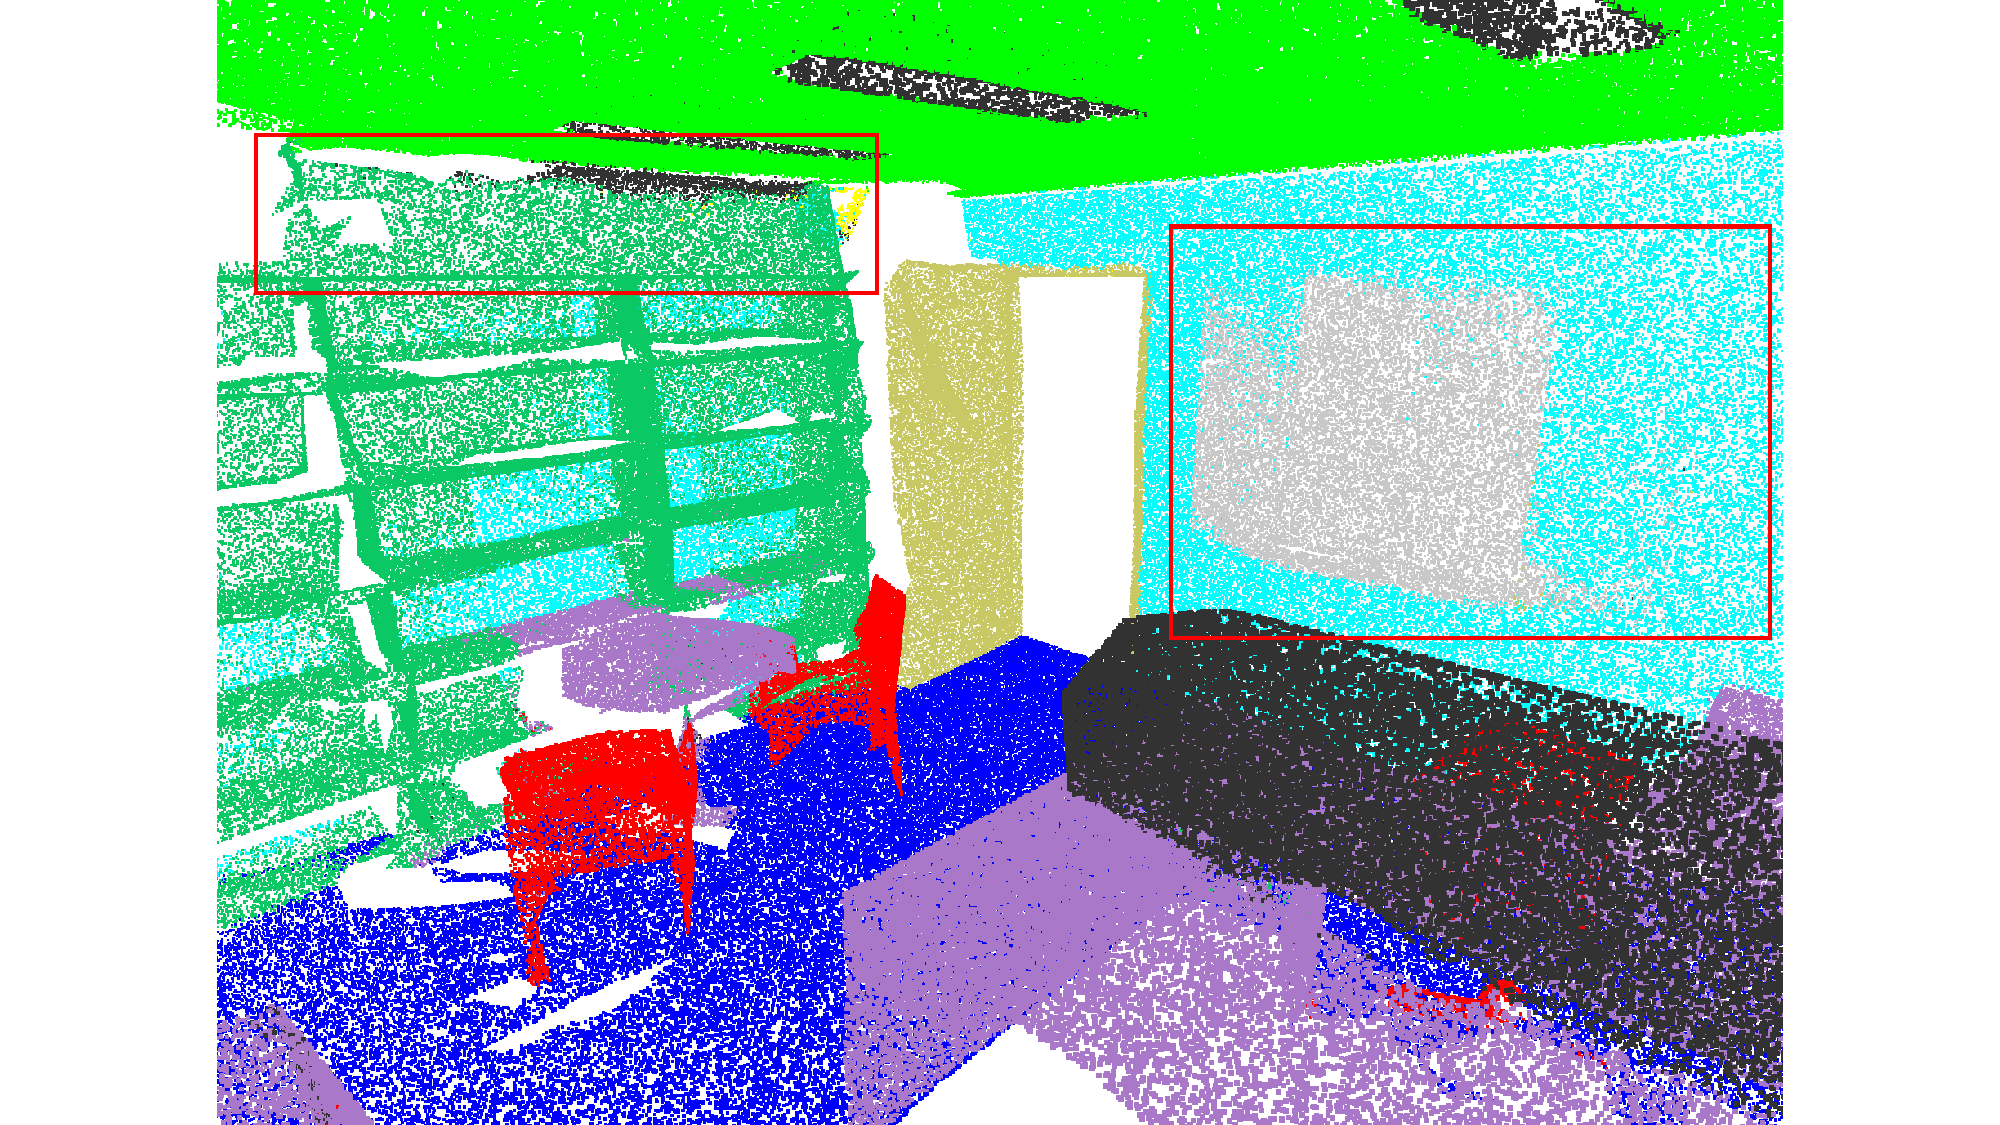
\includegraphics[width=\textwidth]{fig/supplement/semantic_segmentation/office_35/IDPT_office_35.pdf}
    \end{minipage}
    \hfill
    \begin{minipage}{0.22\textwidth}
        \centering
        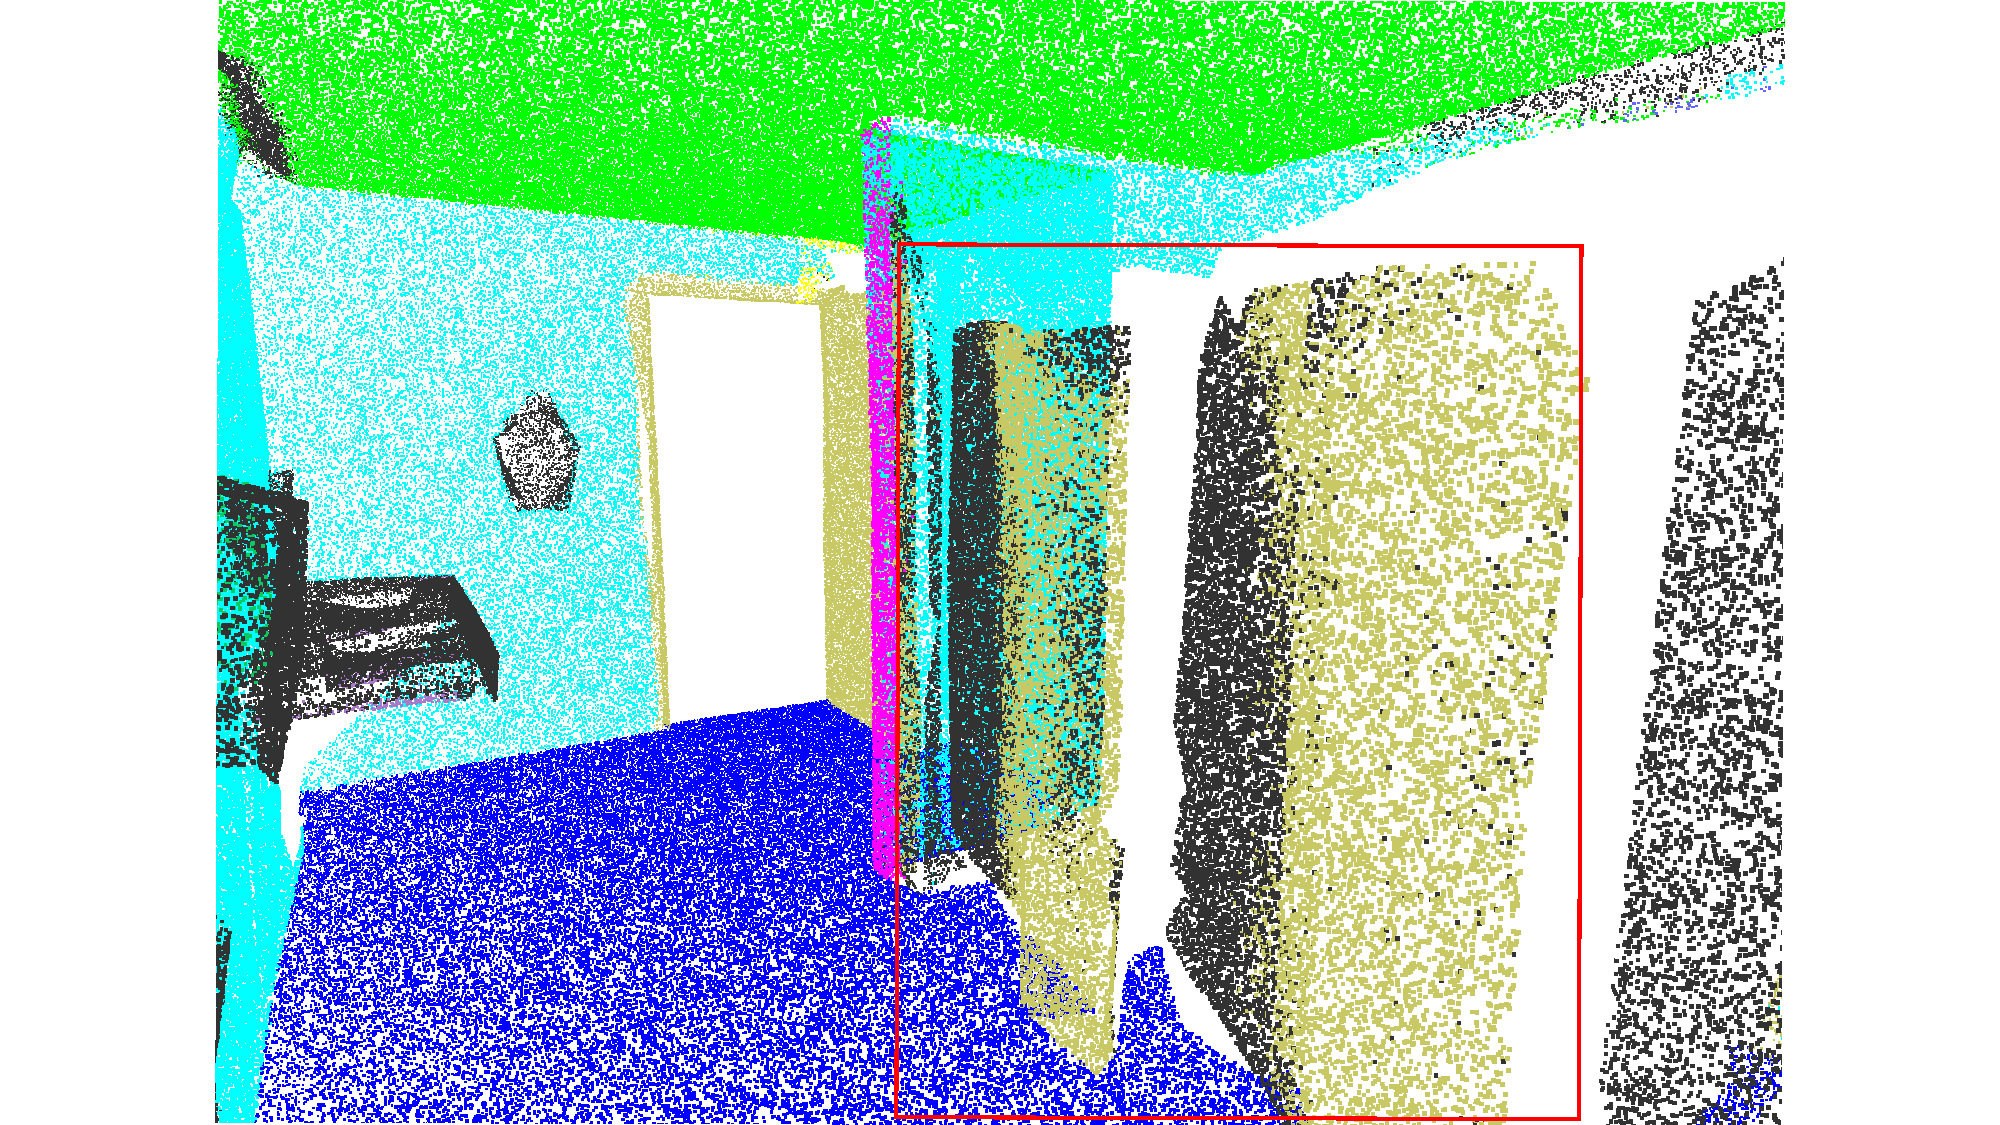
\includegraphics[width=\textwidth]{fig/supplement/semantic_segmentation/wc_2/IDPT_wc_2.pdf}
    \end{minipage}
    \hfill

    % 换行
    \vspace{0.5em}

    % 第四行左侧的竖排标签
    \begin{minipage}{0.09\textwidth}
        \centering
        PPT
    \end{minipage}
    \hfill
    % 第四行图片
    \begin{minipage}{0.22\textwidth}
        \centering
        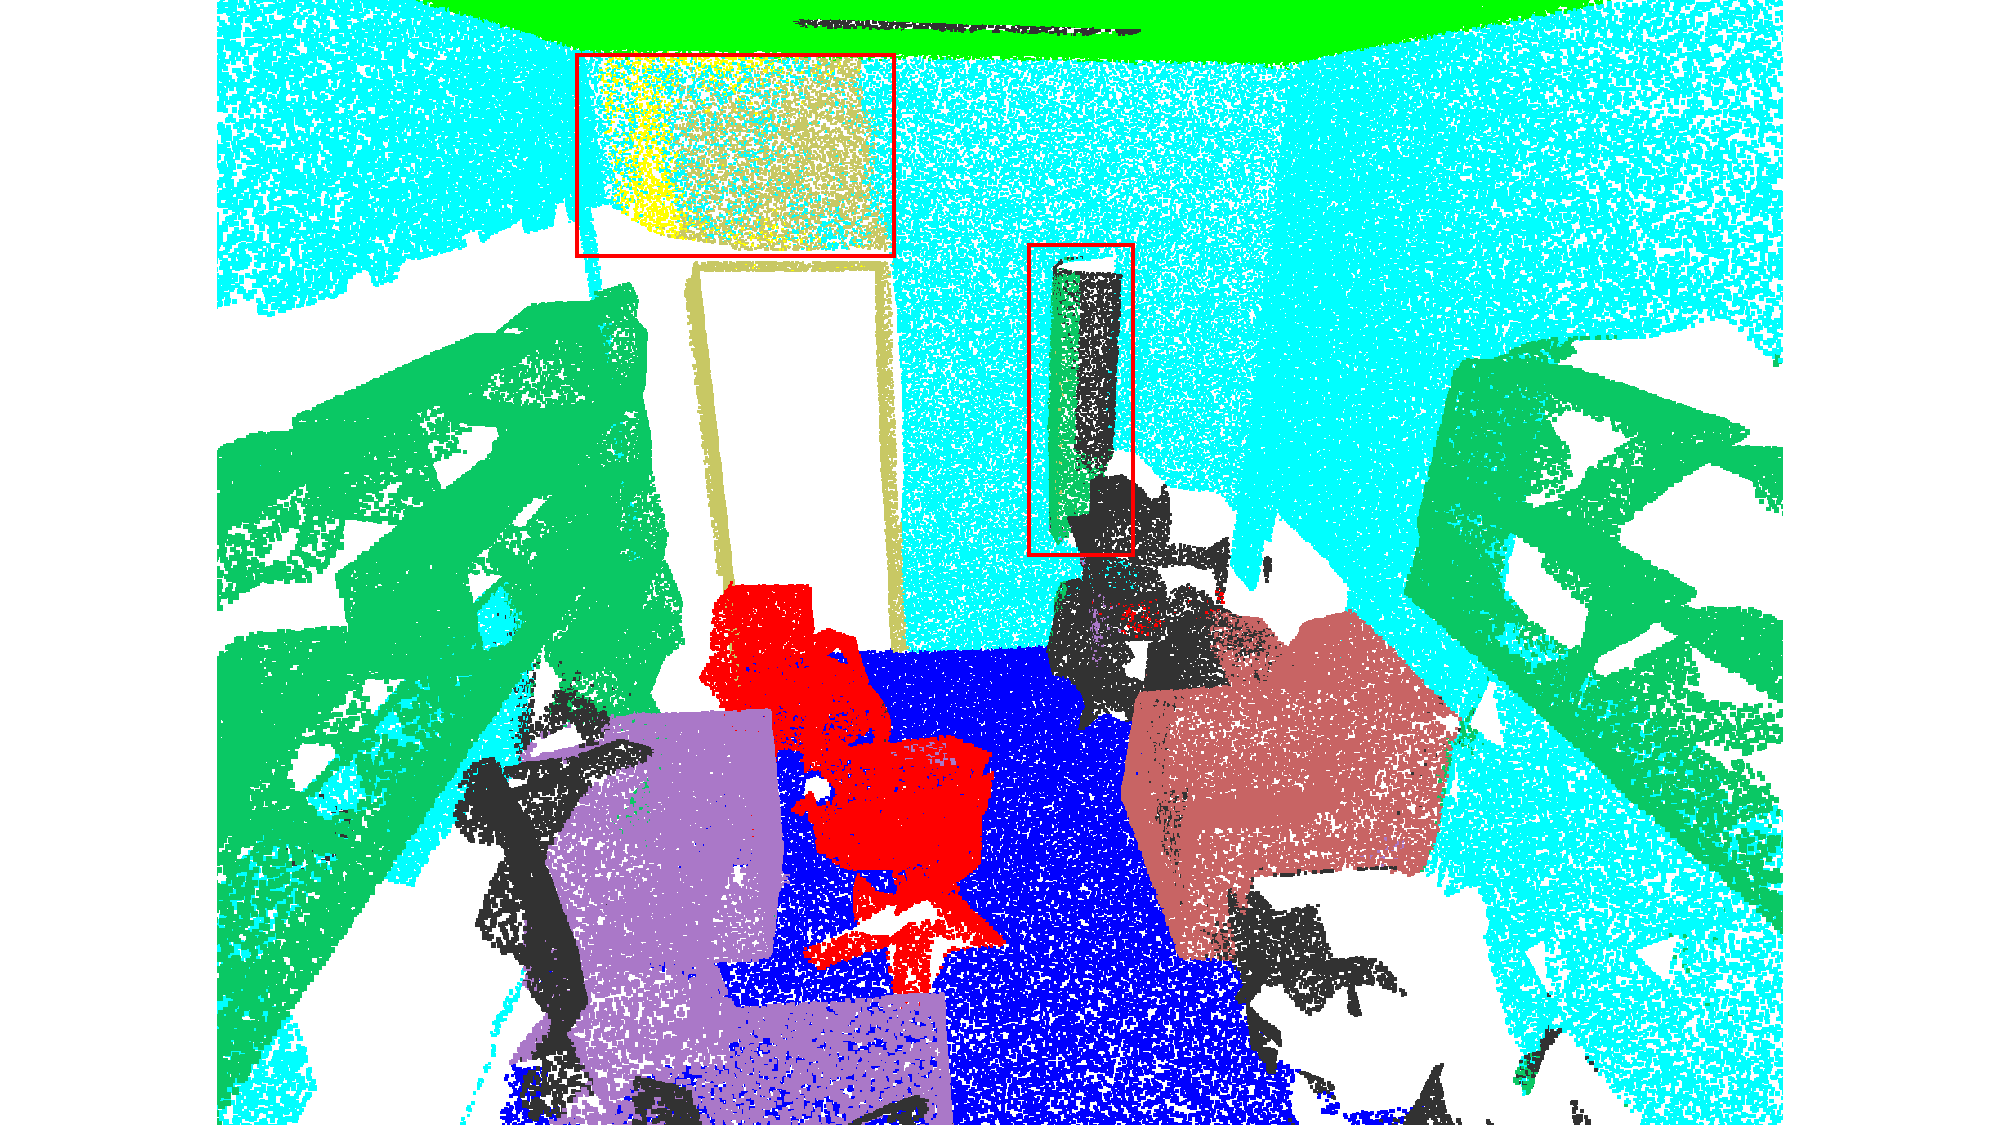
\includegraphics[width=\textwidth]{fig/supplement/semantic_segmentation/office_9/PPT_office_9.pdf}
    \end{minipage}
    \hfill
     \begin{minipage}{0.22\textwidth}
        \centering
        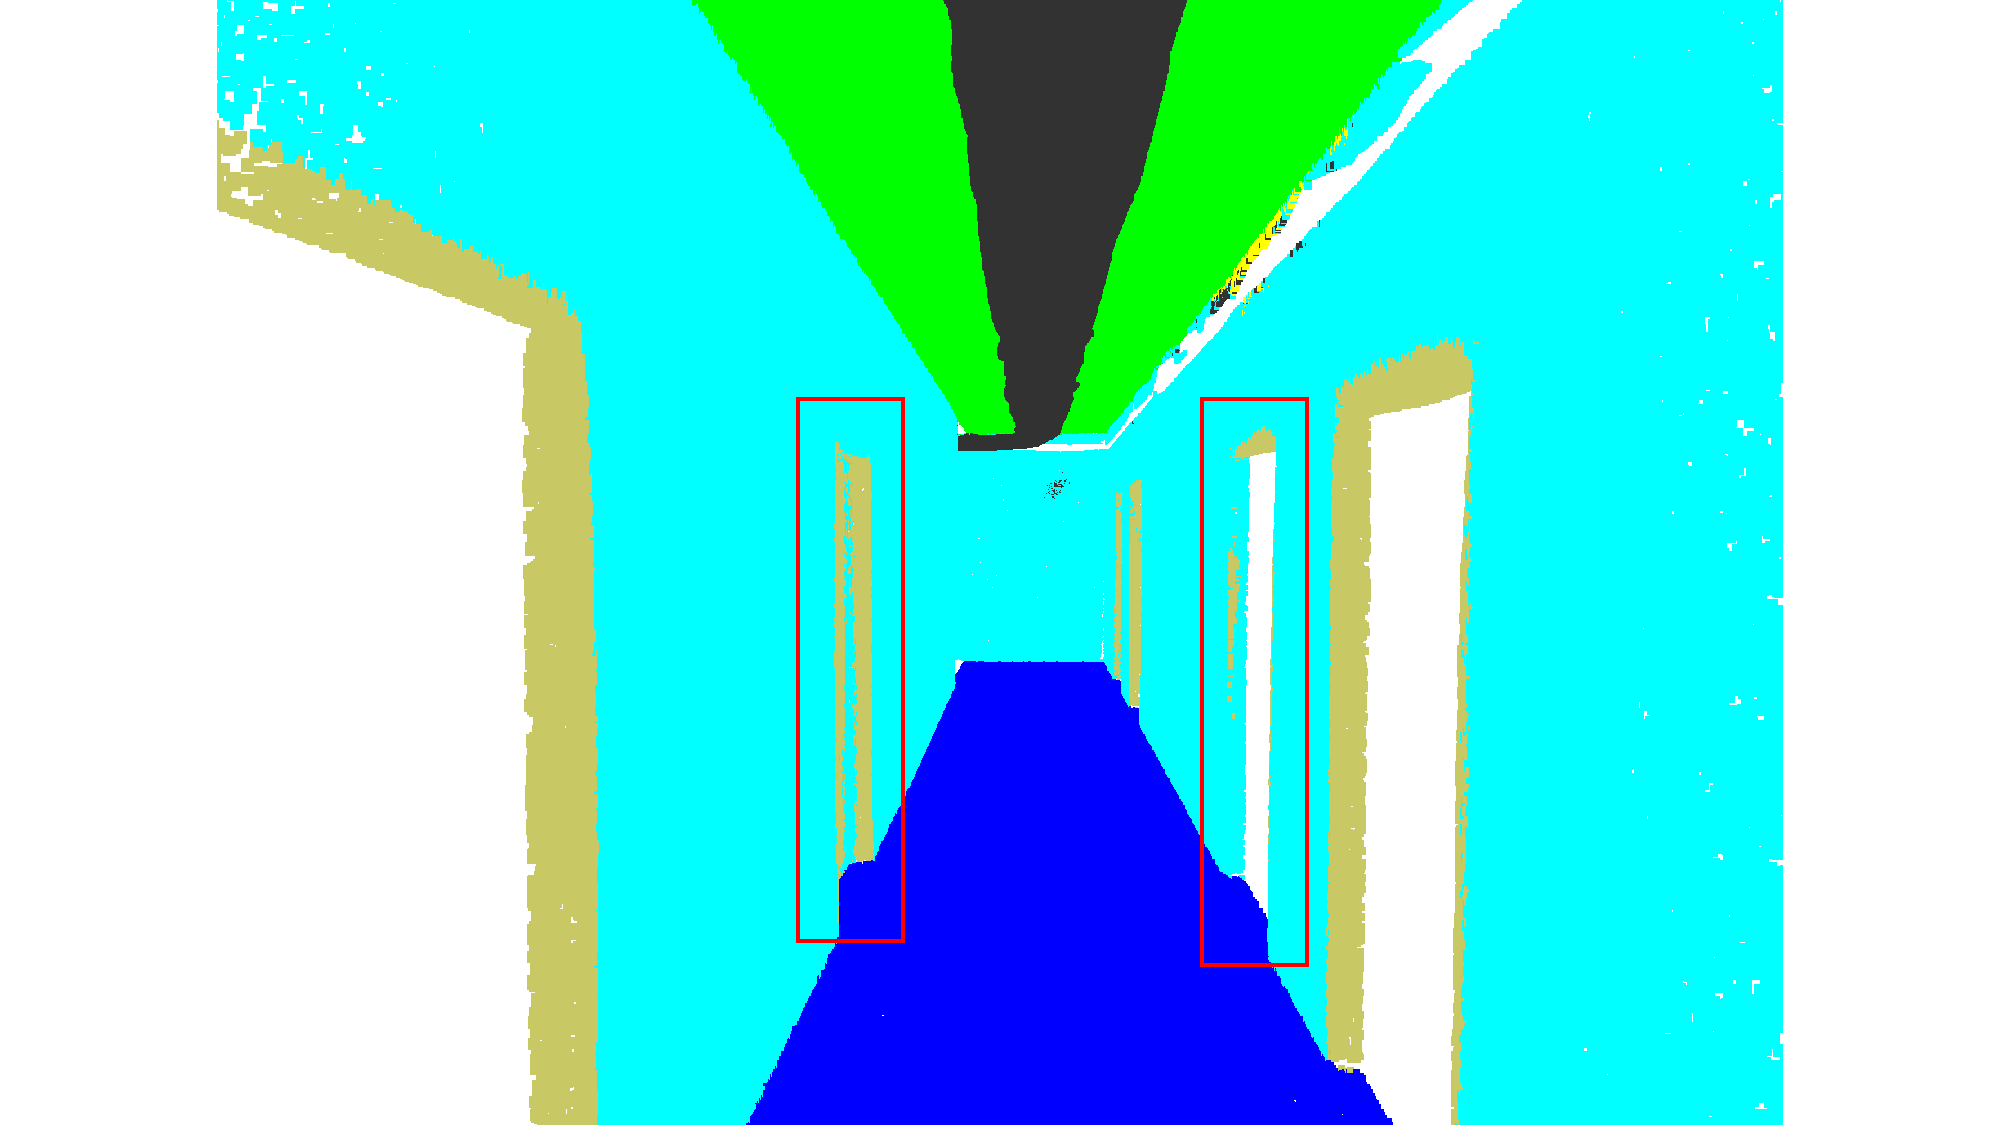
\includegraphics[width=\textwidth]{fig/supplement/semantic_segmentation/hallway_10/PPT_hallway_10.pdf}
    \end{minipage}
    \hfill
    \begin{minipage}{0.22\textwidth}
        \centering
        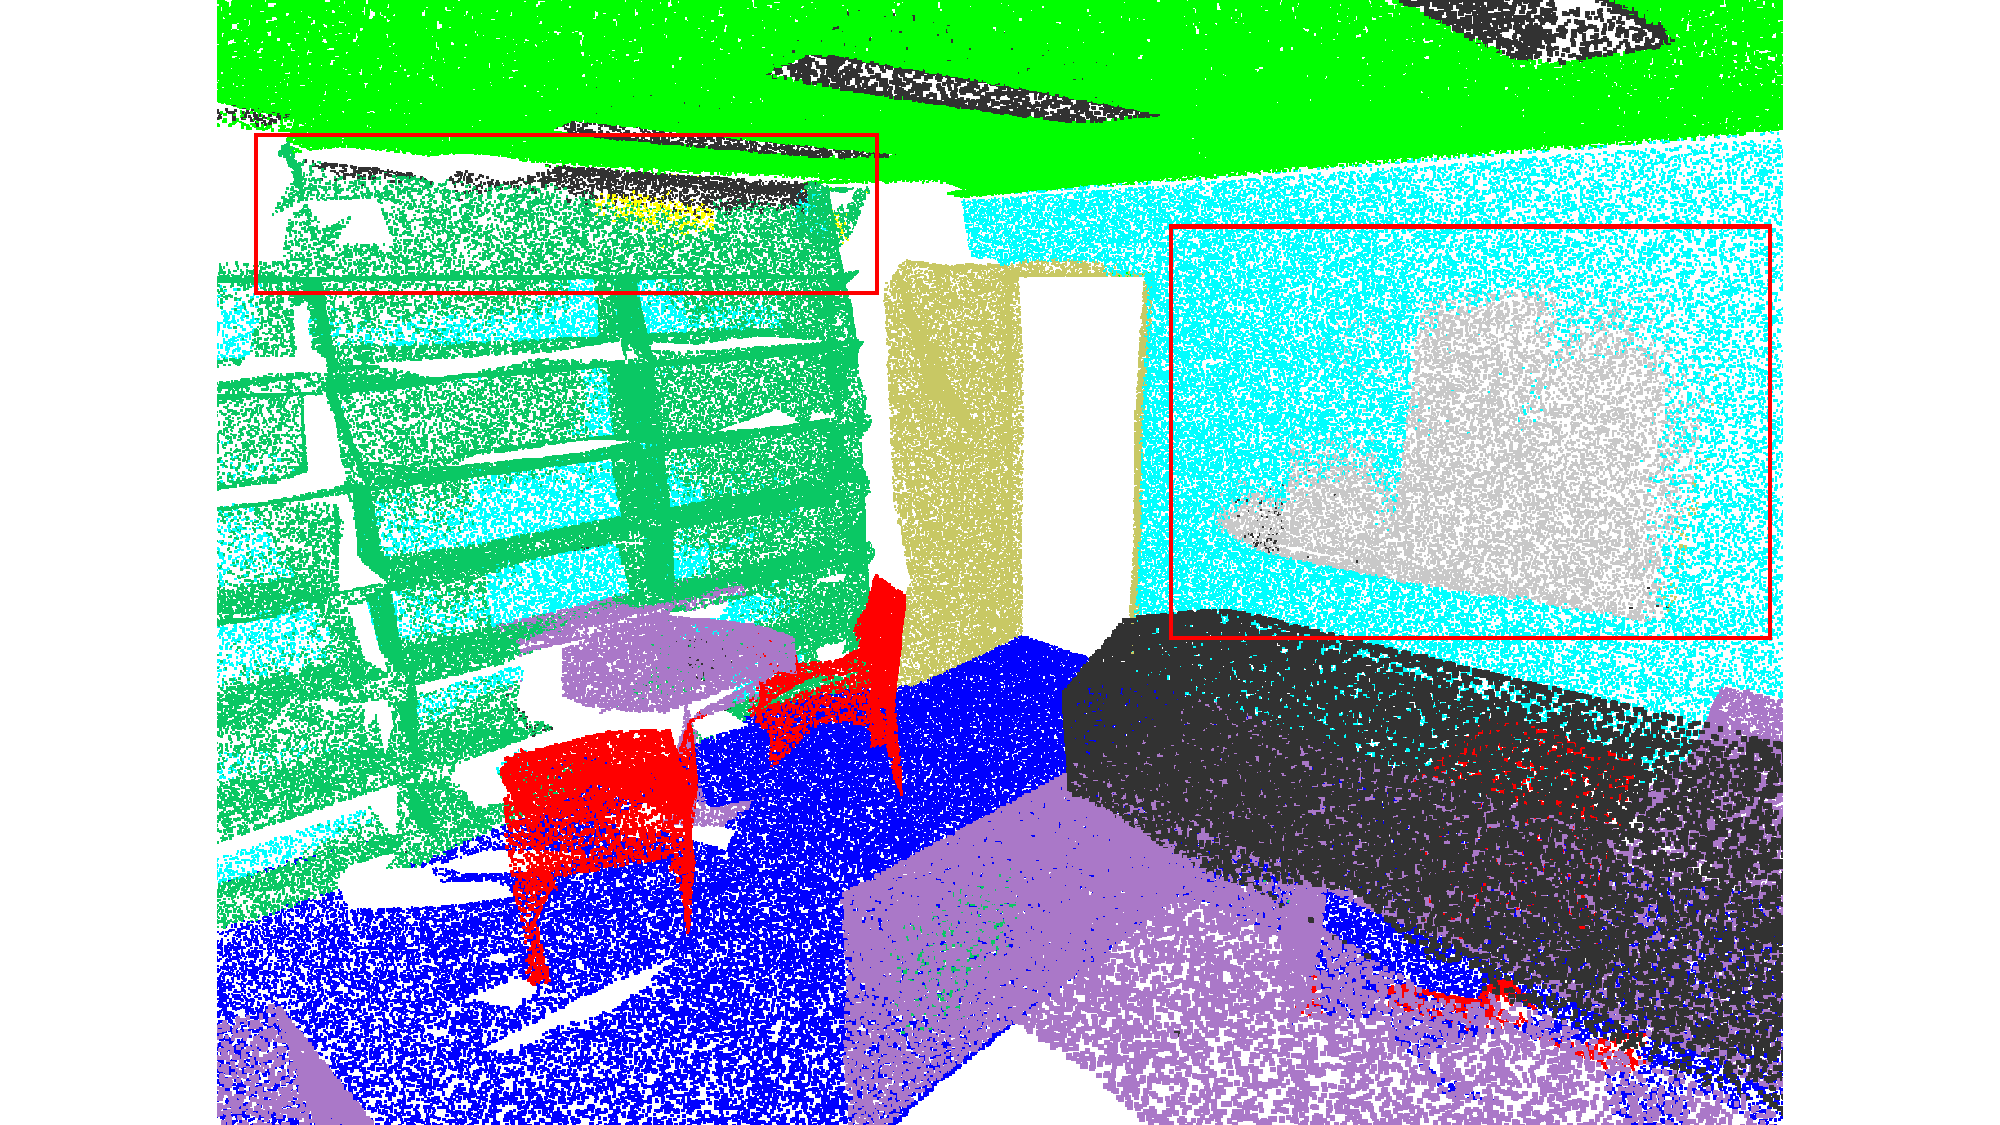
\includegraphics[width=\textwidth]{fig/supplement/semantic_segmentation/office_35/PPT_office_35.pdf}
    \end{minipage}
    \hfill
    \begin{minipage}{0.22\textwidth}
        \centering
        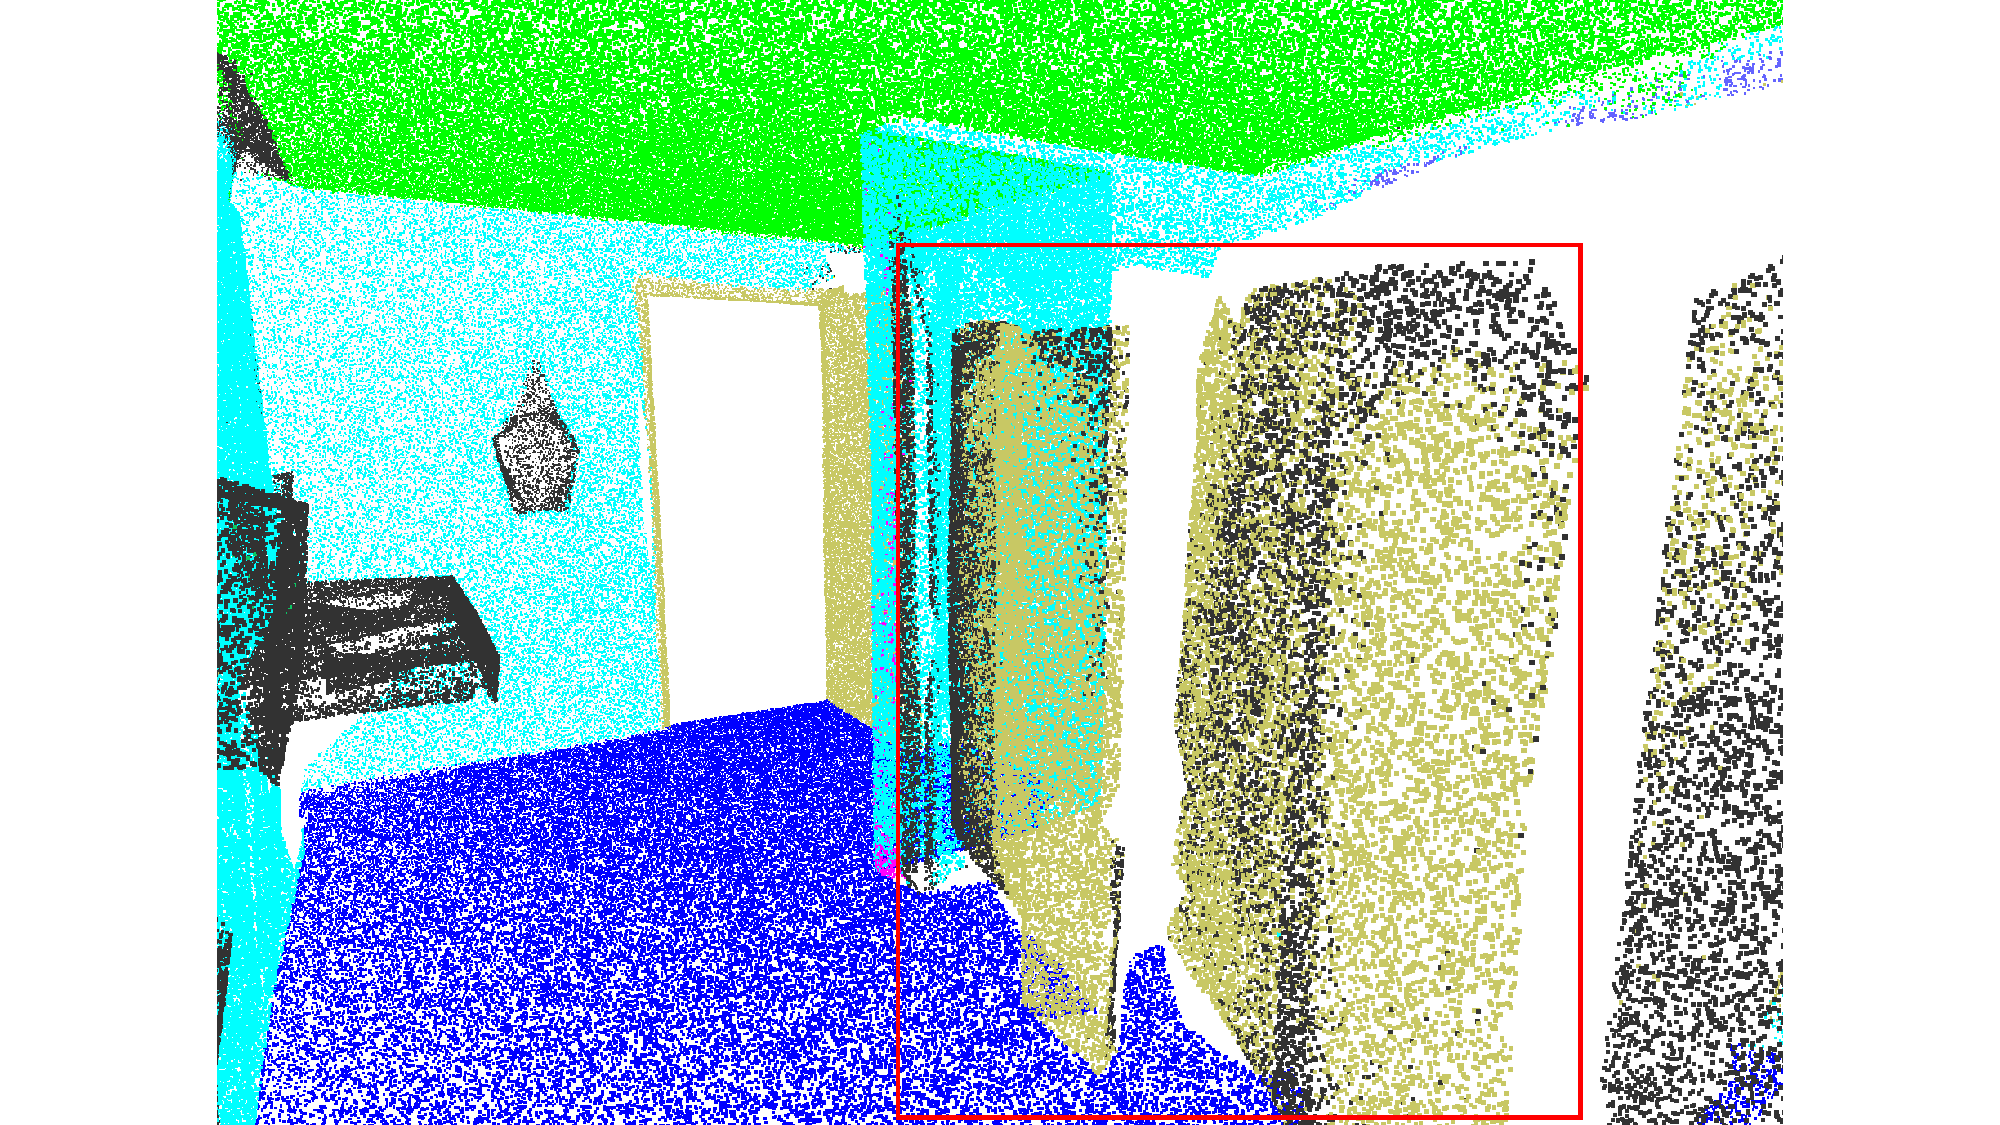
\includegraphics[width=\textwidth]{fig/supplement/semantic_segmentation/wc_2/PPT_wc_2.pdf}
    \end{minipage}
    \hfill

    % 换行
    \vspace{0.5em}

    % 第五行左侧的竖排标签
    \begin{minipage}{0.09\textwidth}
        \centering
        PointGST
    \end{minipage}
    \hfill
    % 第五行图片
    \begin{minipage}{0.22\textwidth}
        \centering
        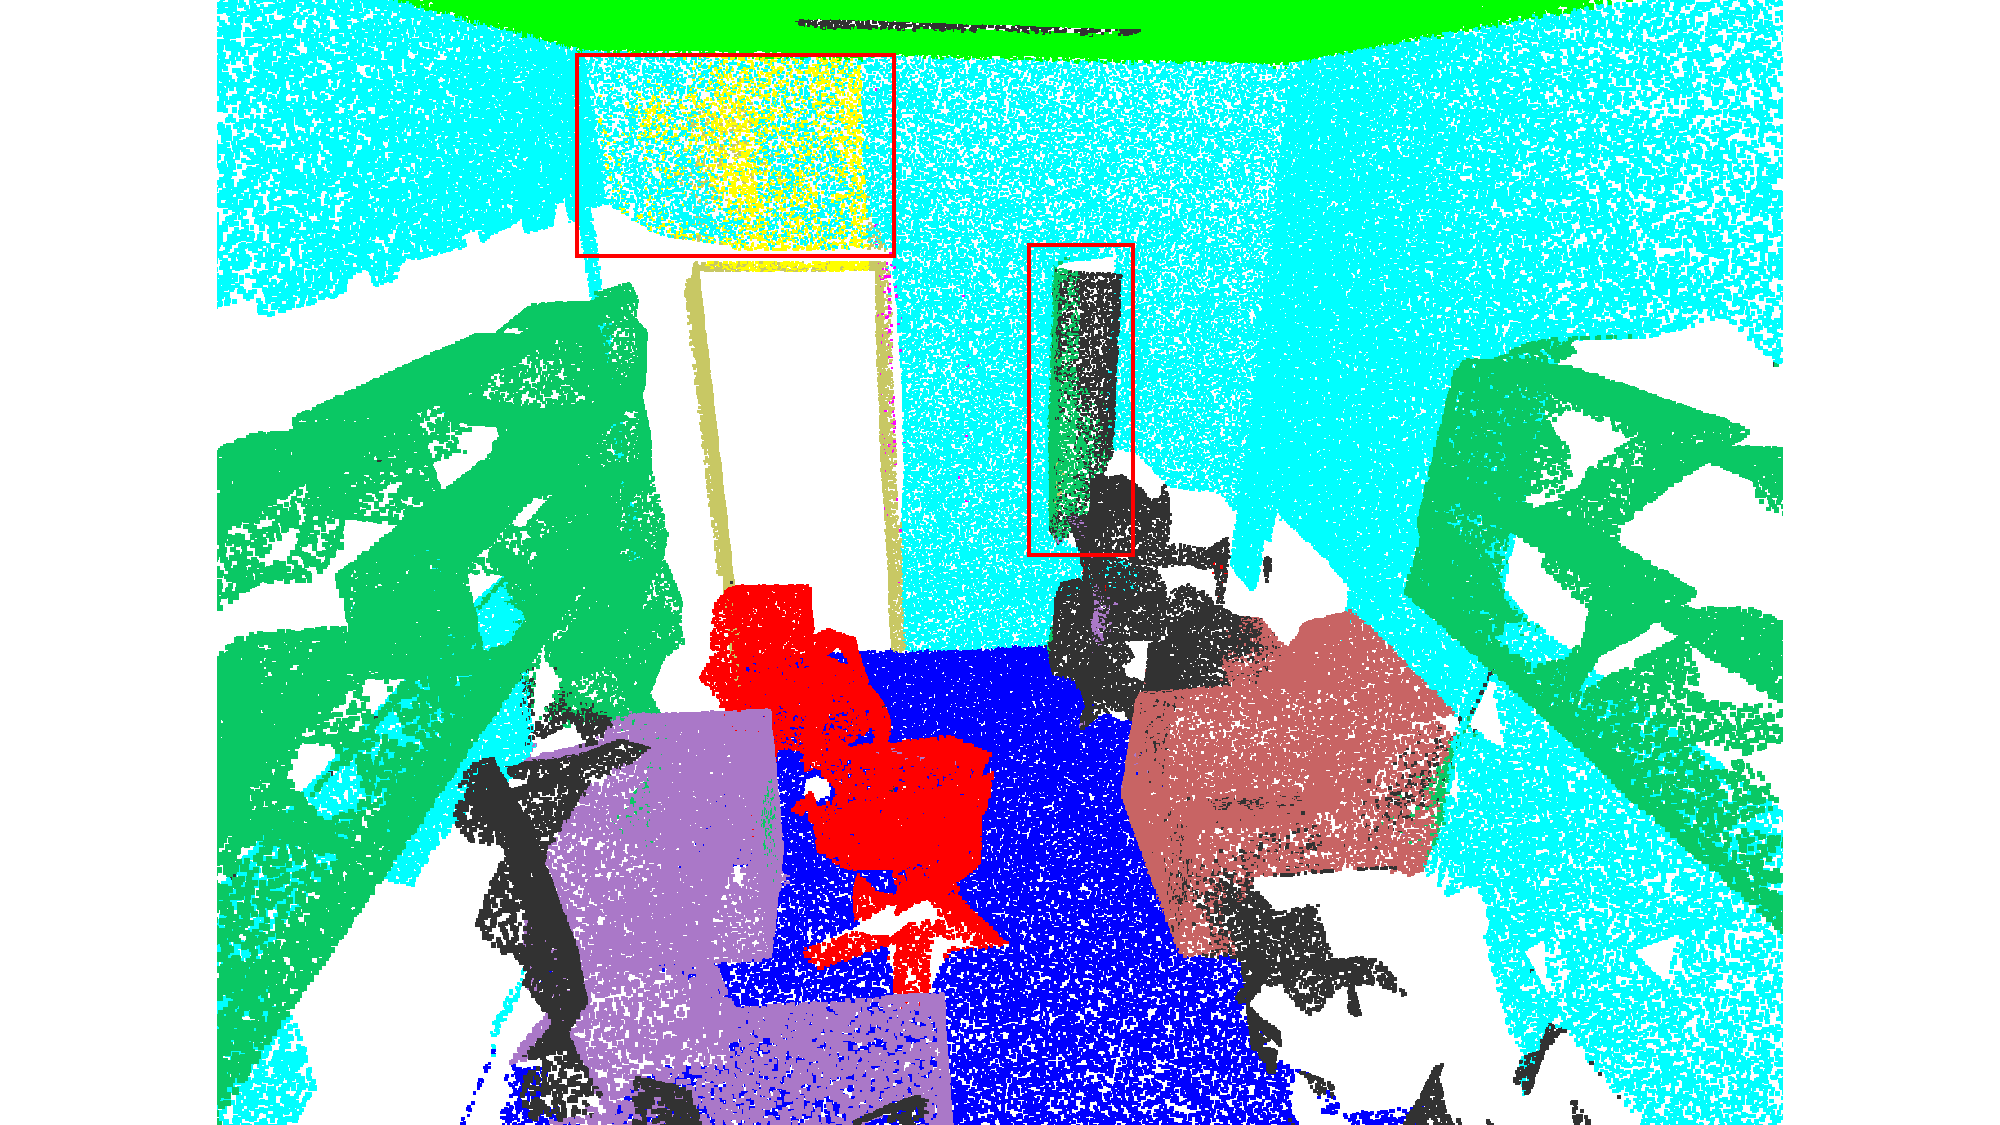
\includegraphics[width=\textwidth]{fig/supplement/semantic_segmentation/office_9/PointGST_office_9.pdf}
    \end{minipage}
    \hfill
    \begin{minipage}{0.22\textwidth}
        \centering
        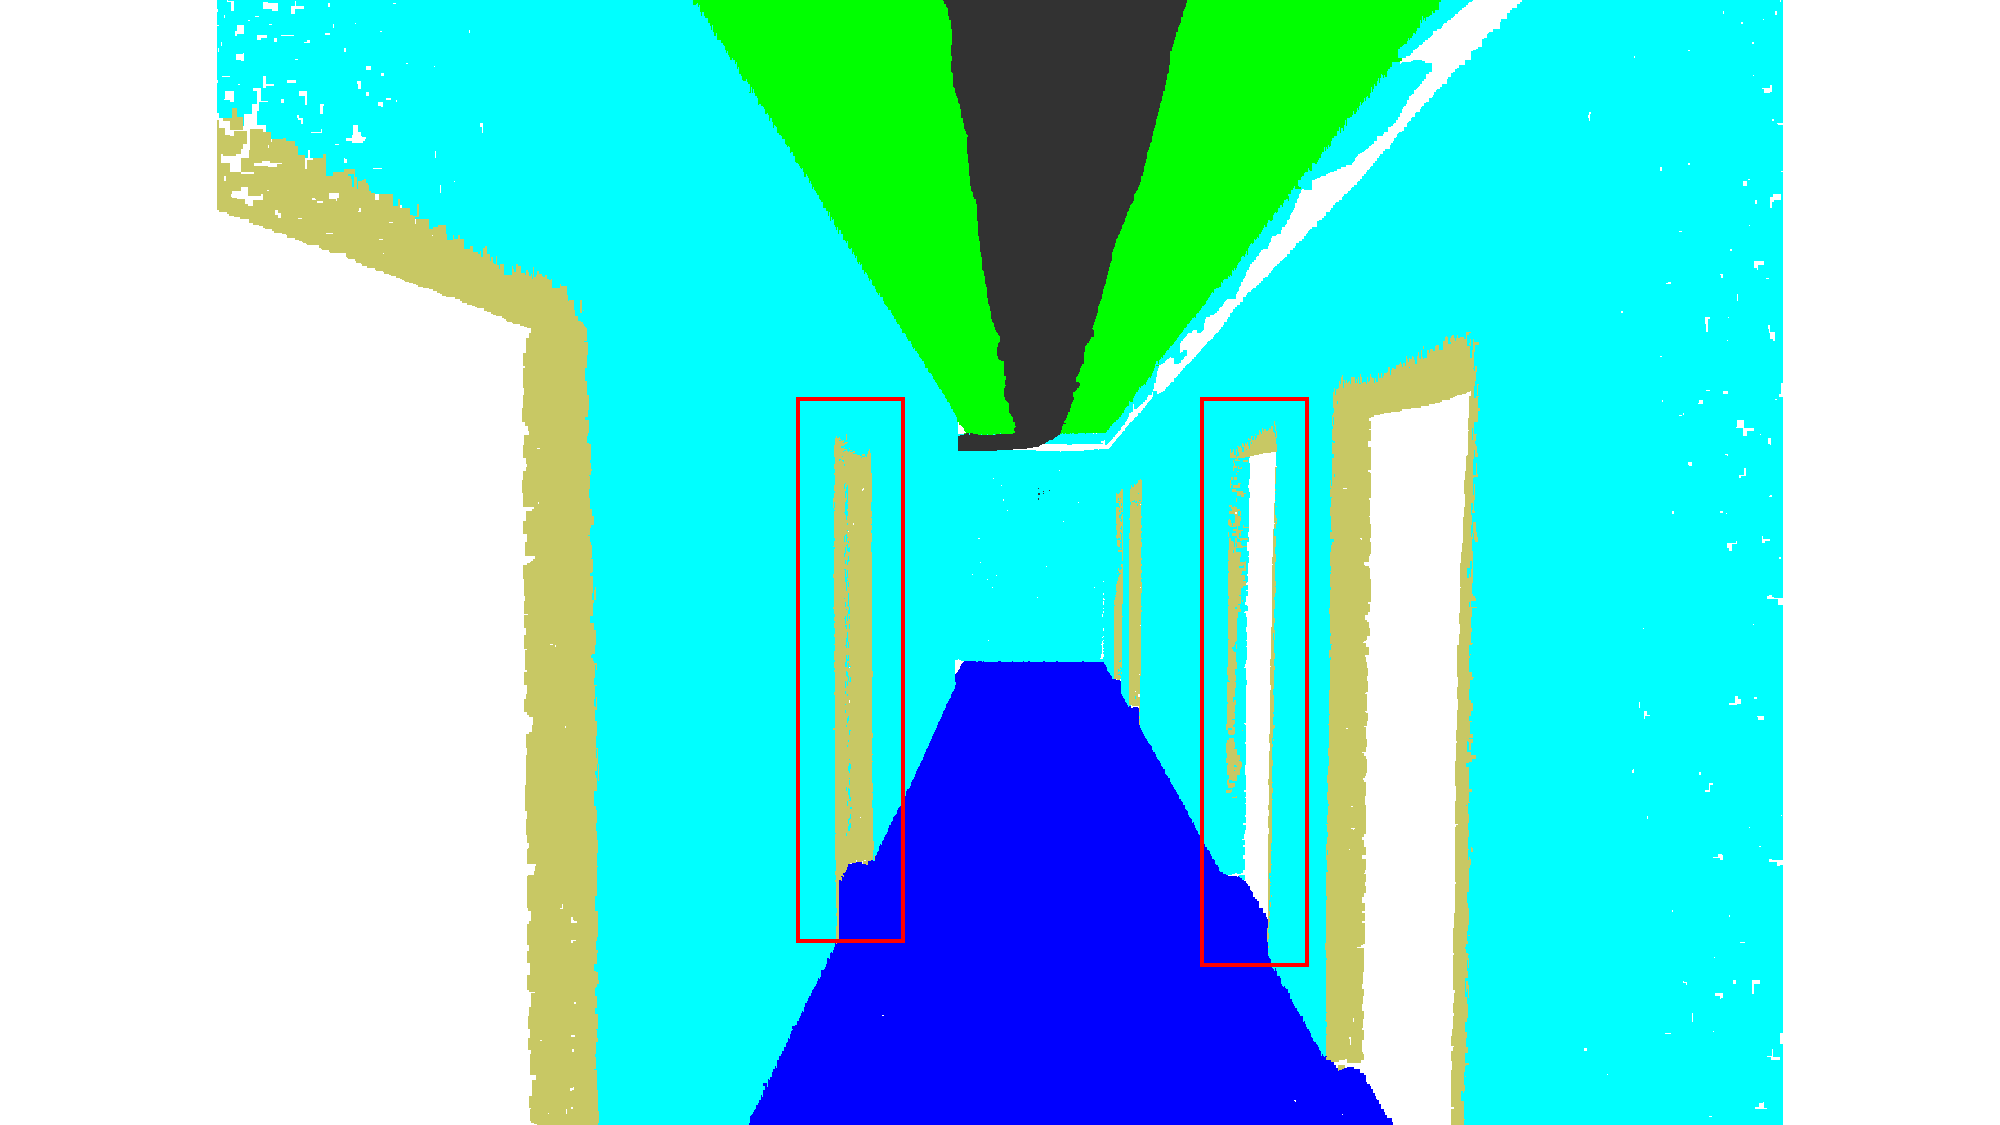
\includegraphics[width=\textwidth]{fig/supplement/semantic_segmentation/hallway_10/PointGST_hallway_10.pdf}
    \end{minipage}
    \hfill
    \begin{minipage}{0.22\textwidth}
        \centering
        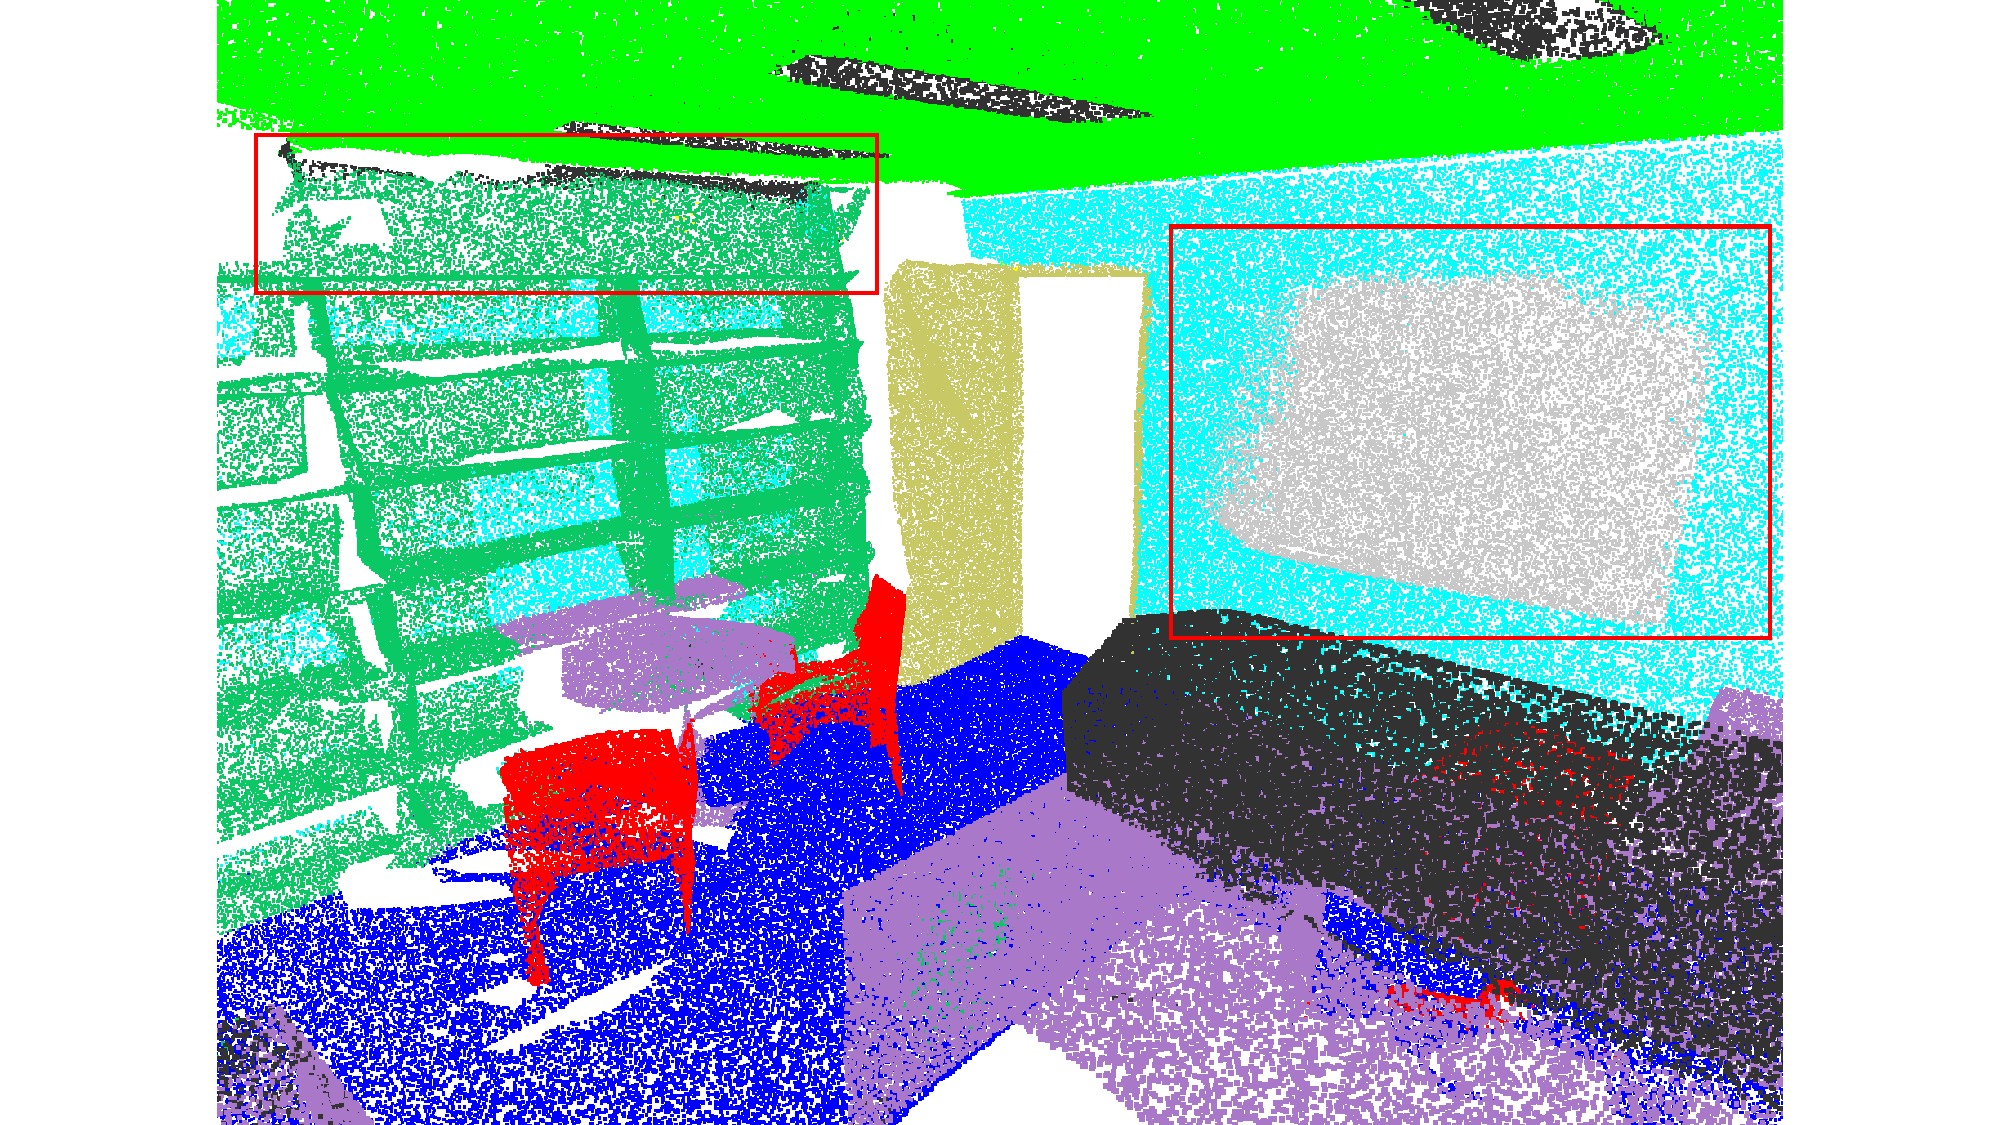
\includegraphics[width=\textwidth]{fig/supplement/semantic_segmentation/office_35/PointGST_office_35.pdf}
    \end{minipage}
    \hfill
    \begin{minipage}{0.22\textwidth}
        \centering
        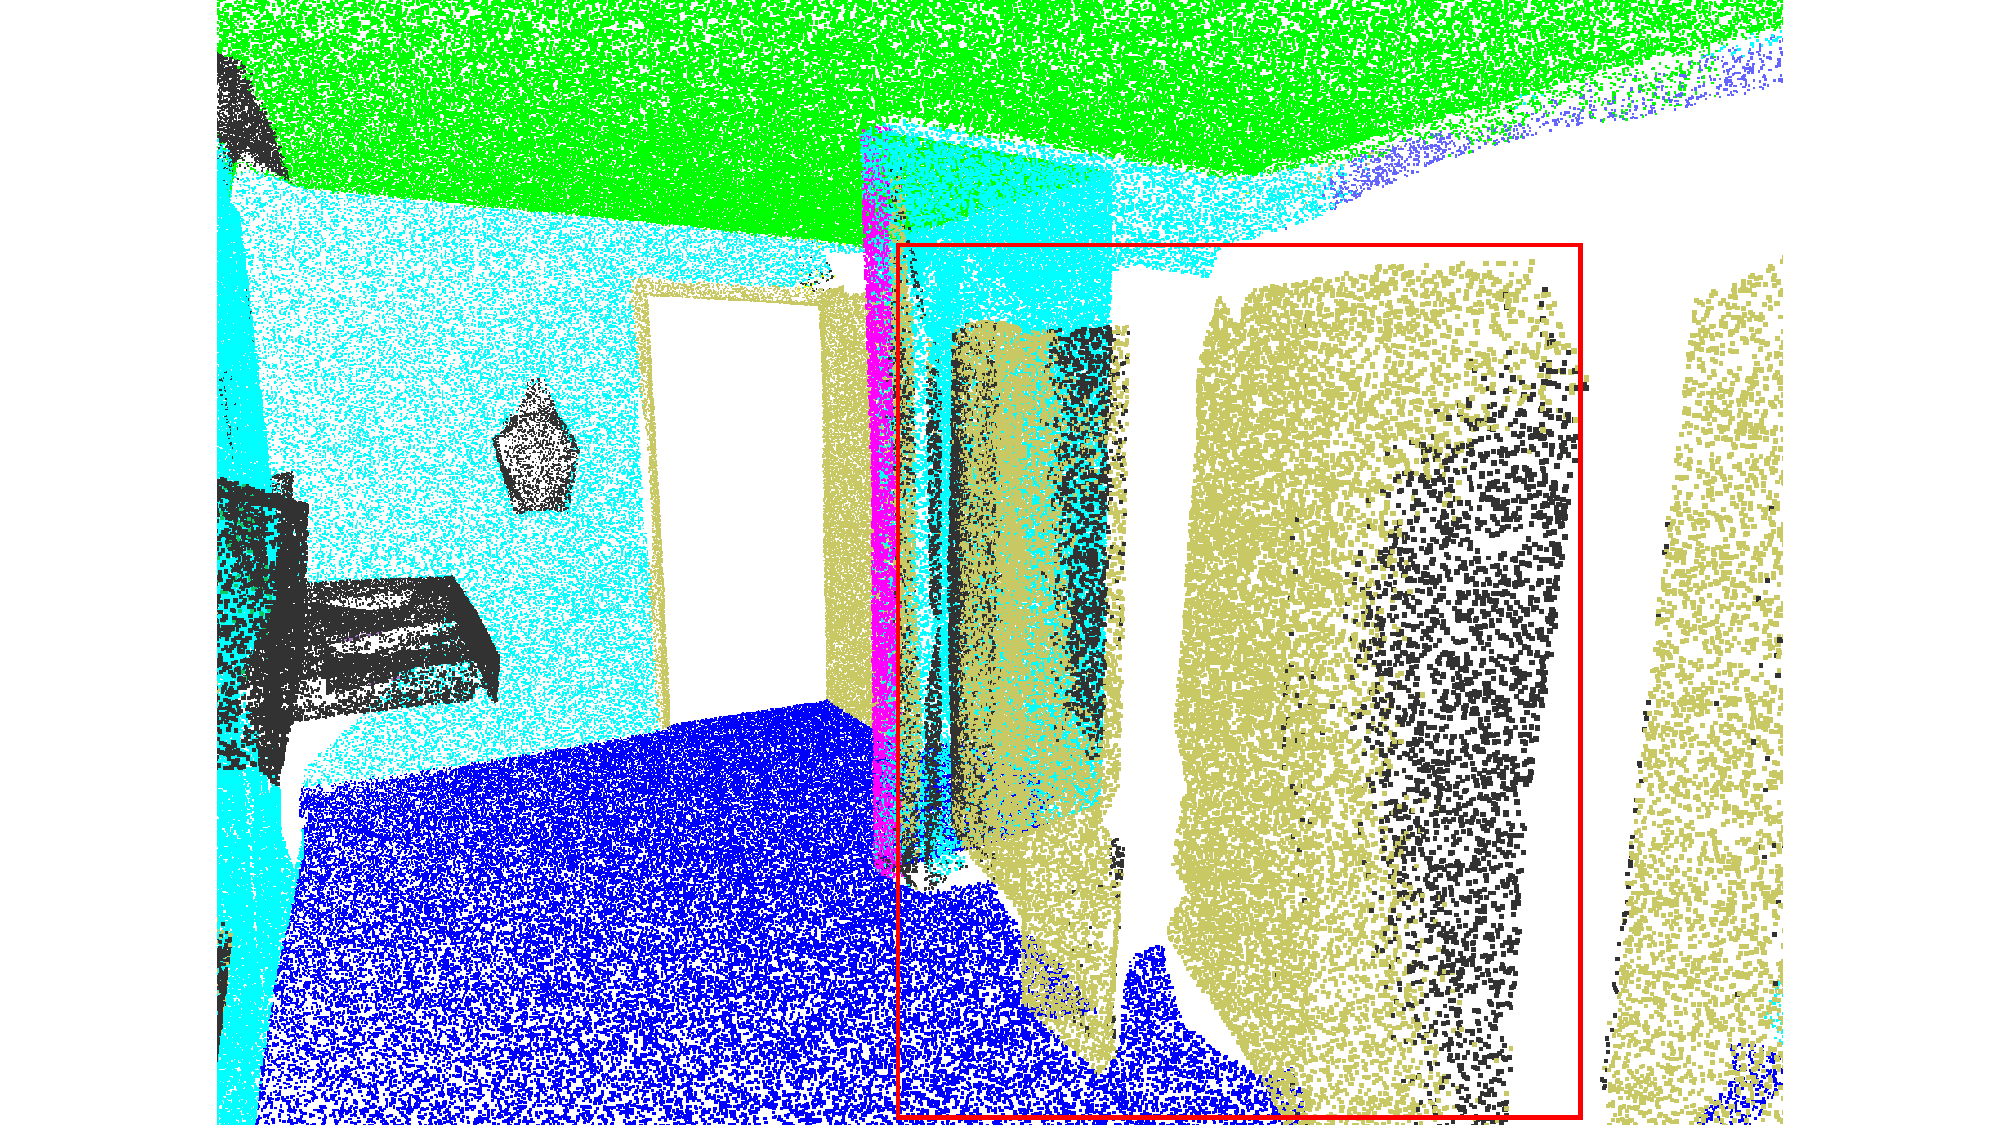
\includegraphics[width=\textwidth]{fig/supplement/semantic_segmentation/wc_2/PointGST_wc_2.pdf}
    \end{minipage}
    \hfill

    % 换行
    \vspace{0.5em}

    % 第六行左侧的竖排标签
    \begin{minipage}{0.09\textwidth}
        \centering
        PLT (Ours)
    \end{minipage}
    \hfill
    % 第六行图片
    \begin{minipage}{0.22\textwidth}
        \centering
        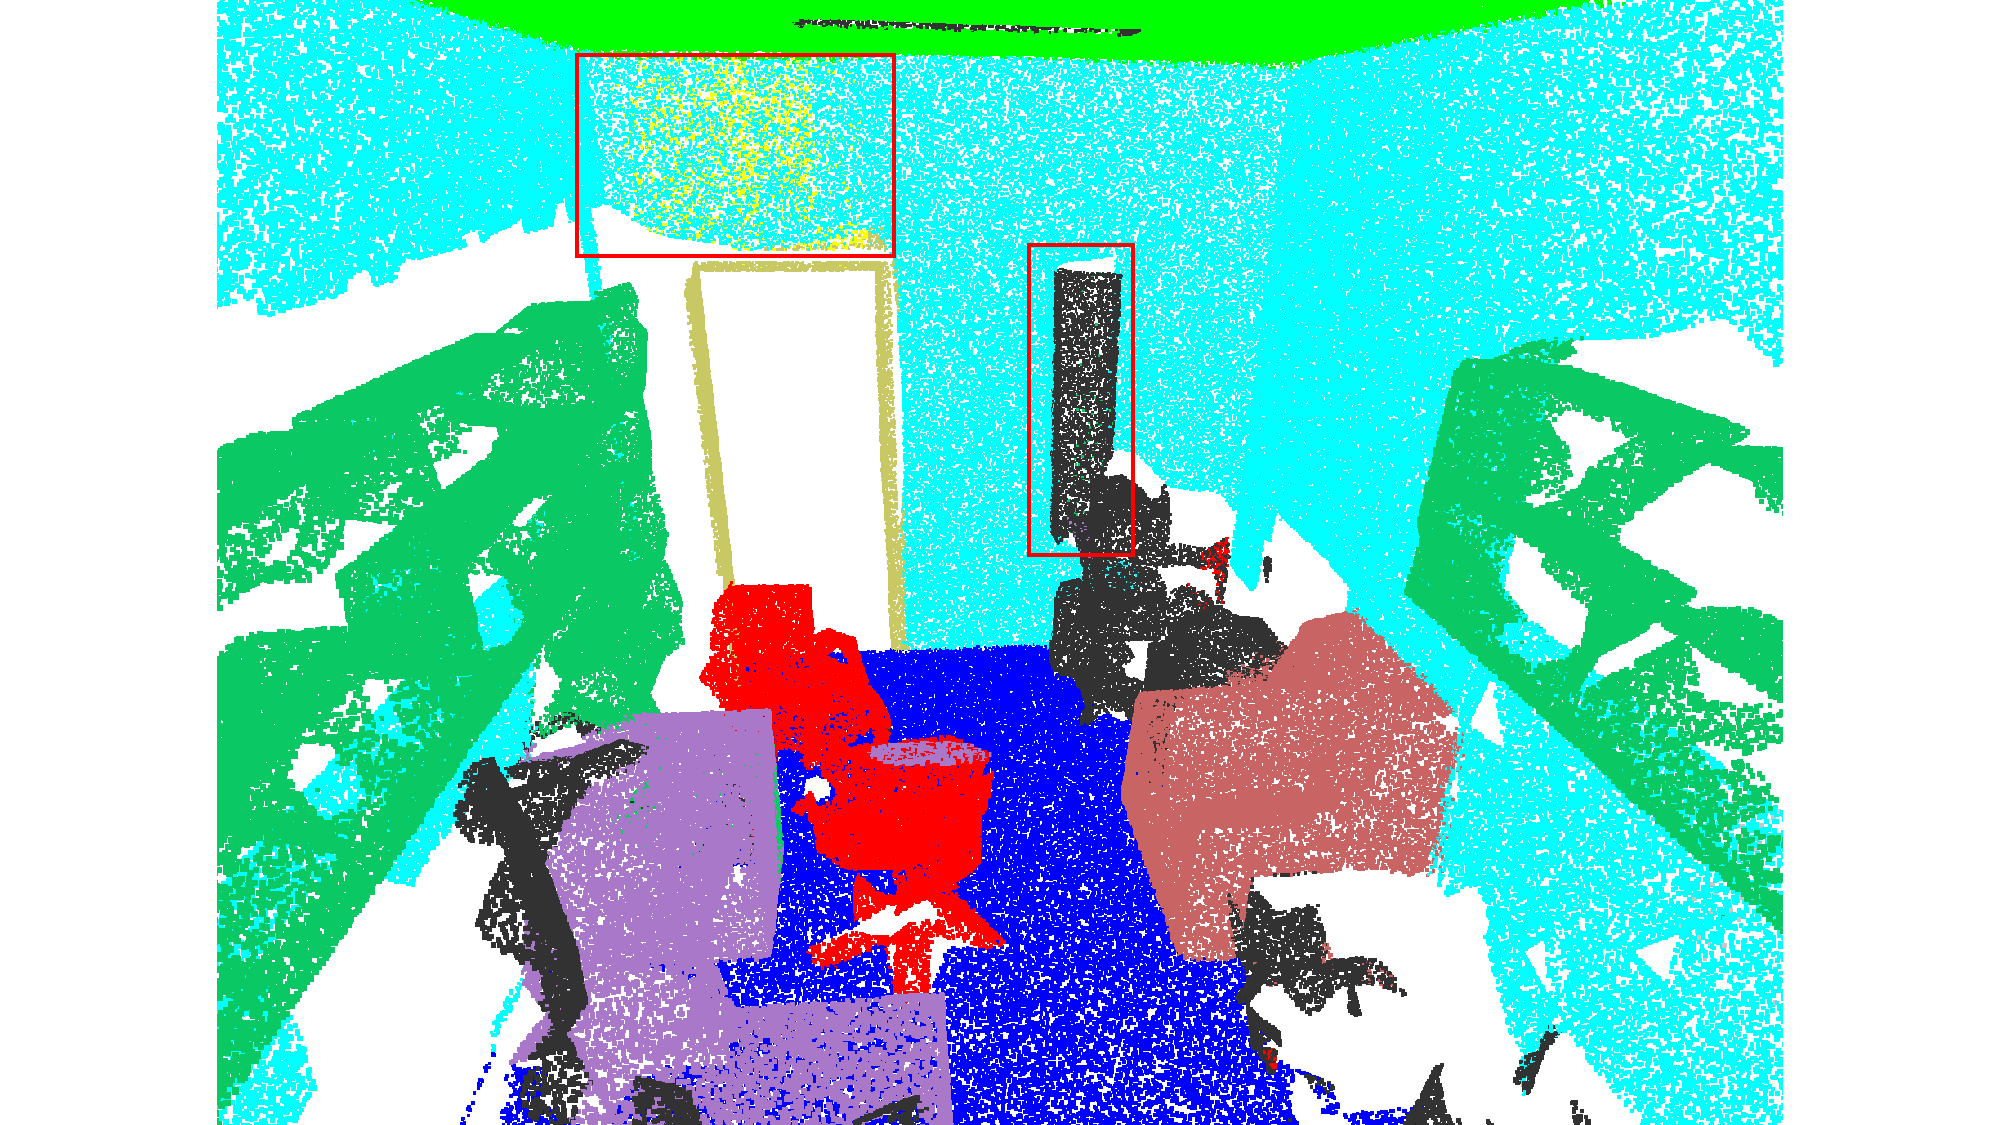
\includegraphics[width=\textwidth]{fig/supplement/semantic_segmentation/office_9/PLT_office_9.pdf}
    \end{minipage}
    \hfill
    \begin{minipage}{0.22\textwidth}
        \centering
        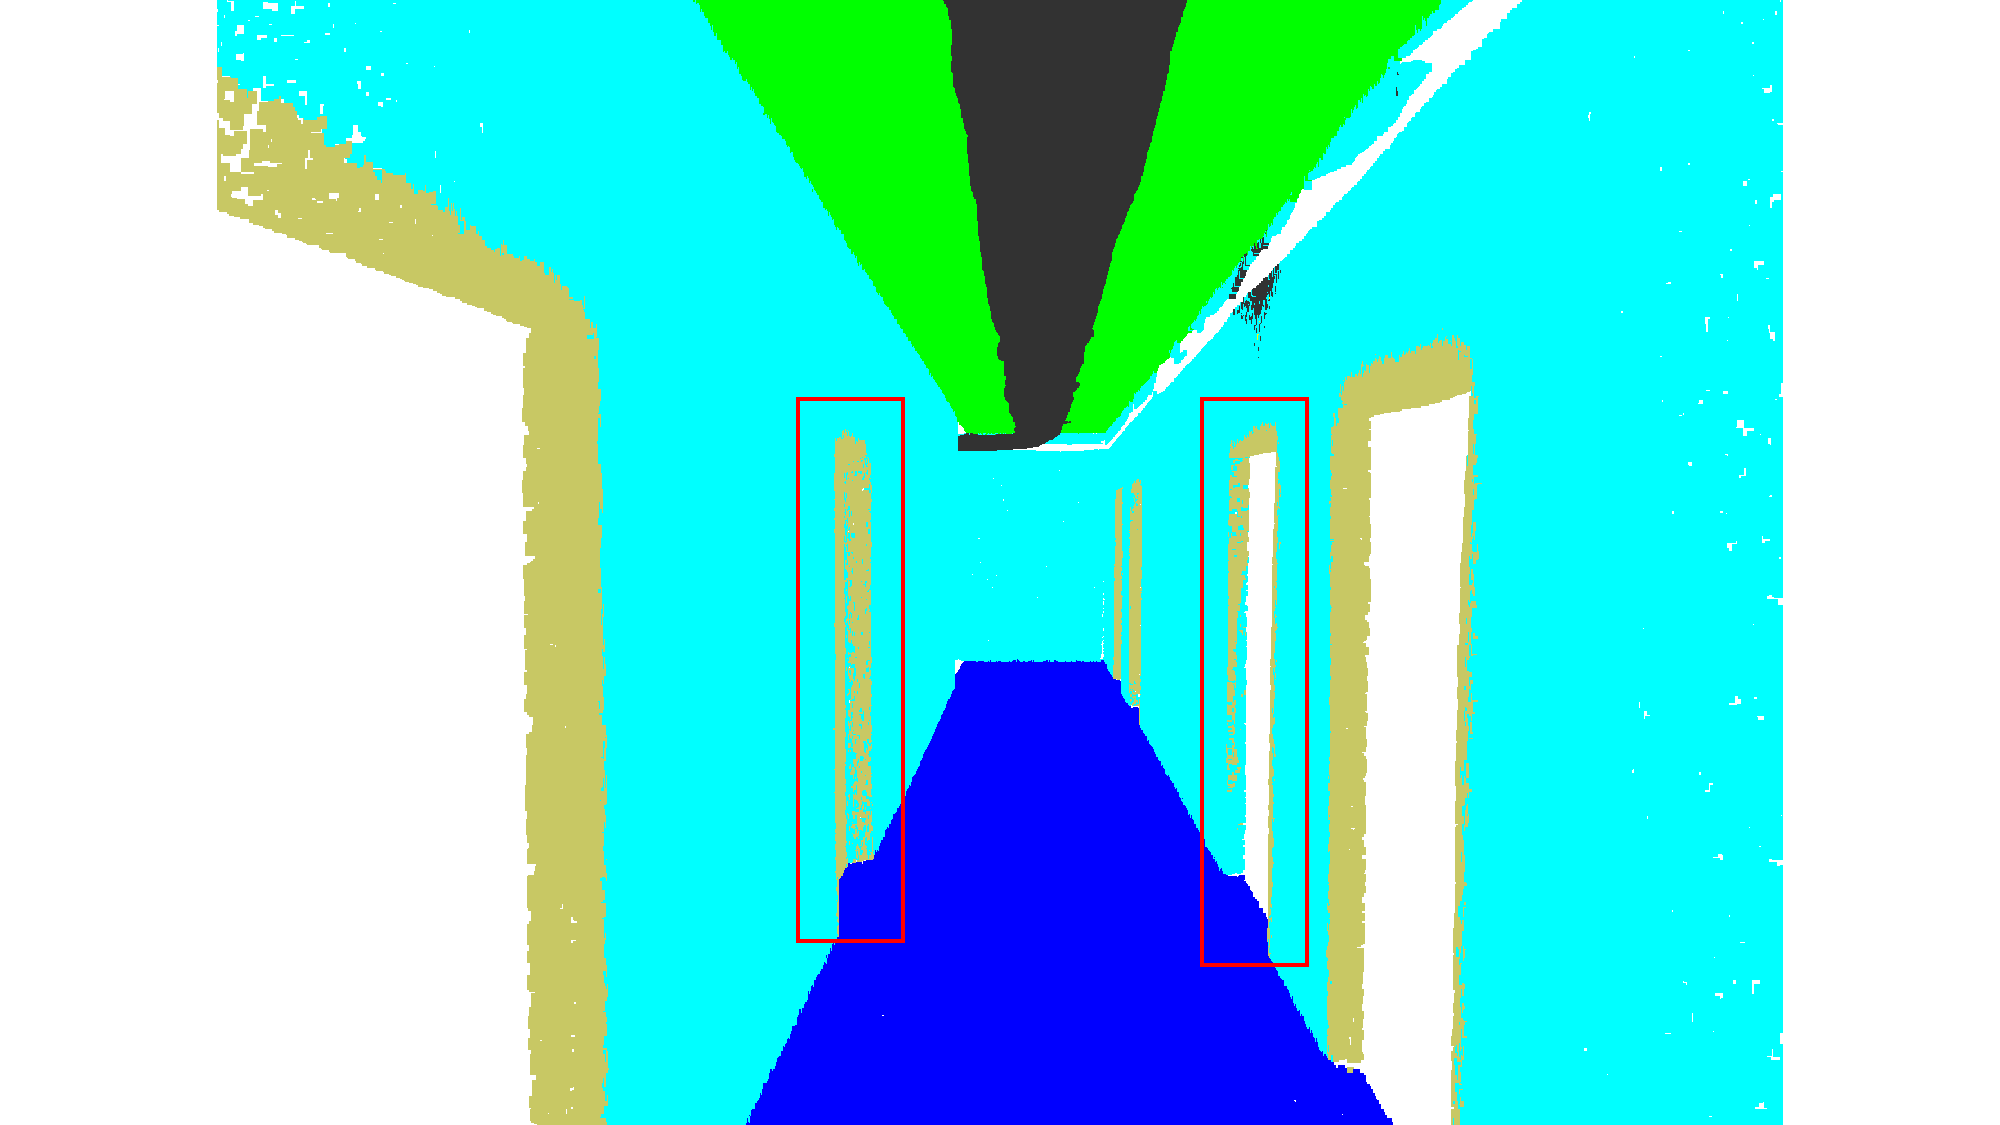
\includegraphics[width=\textwidth]{fig/supplement/semantic_segmentation/hallway_10/PLT_hallway_10.pdf}
    \end{minipage}
    \hfill
    \begin{minipage}{0.22\textwidth}
        \centering
        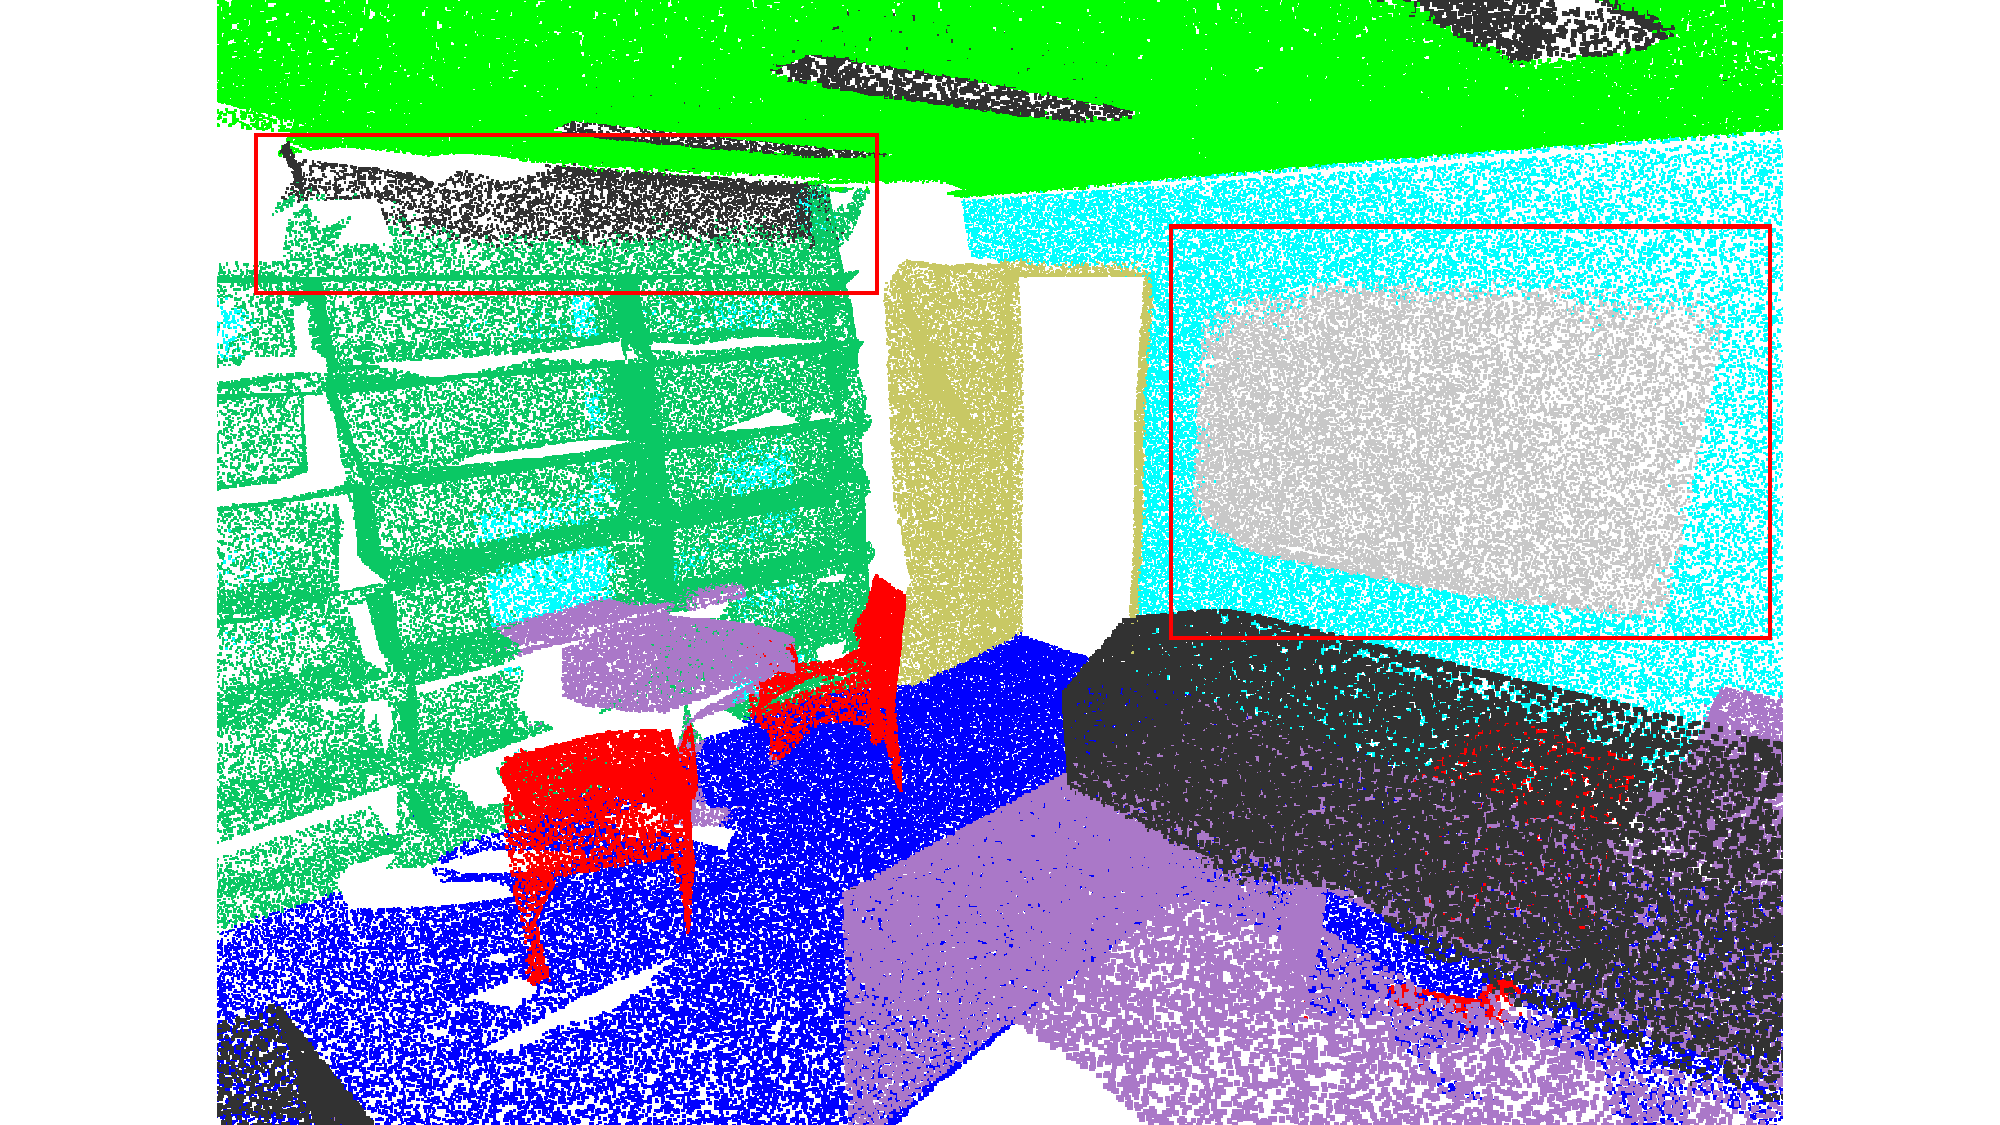
\includegraphics[width=\textwidth]{fig/supplement/semantic_segmentation/office_35/PLT_office_35.pdf}
    \end{minipage}
    \hfill
    \begin{minipage}{0.22\textwidth}
        \centering
        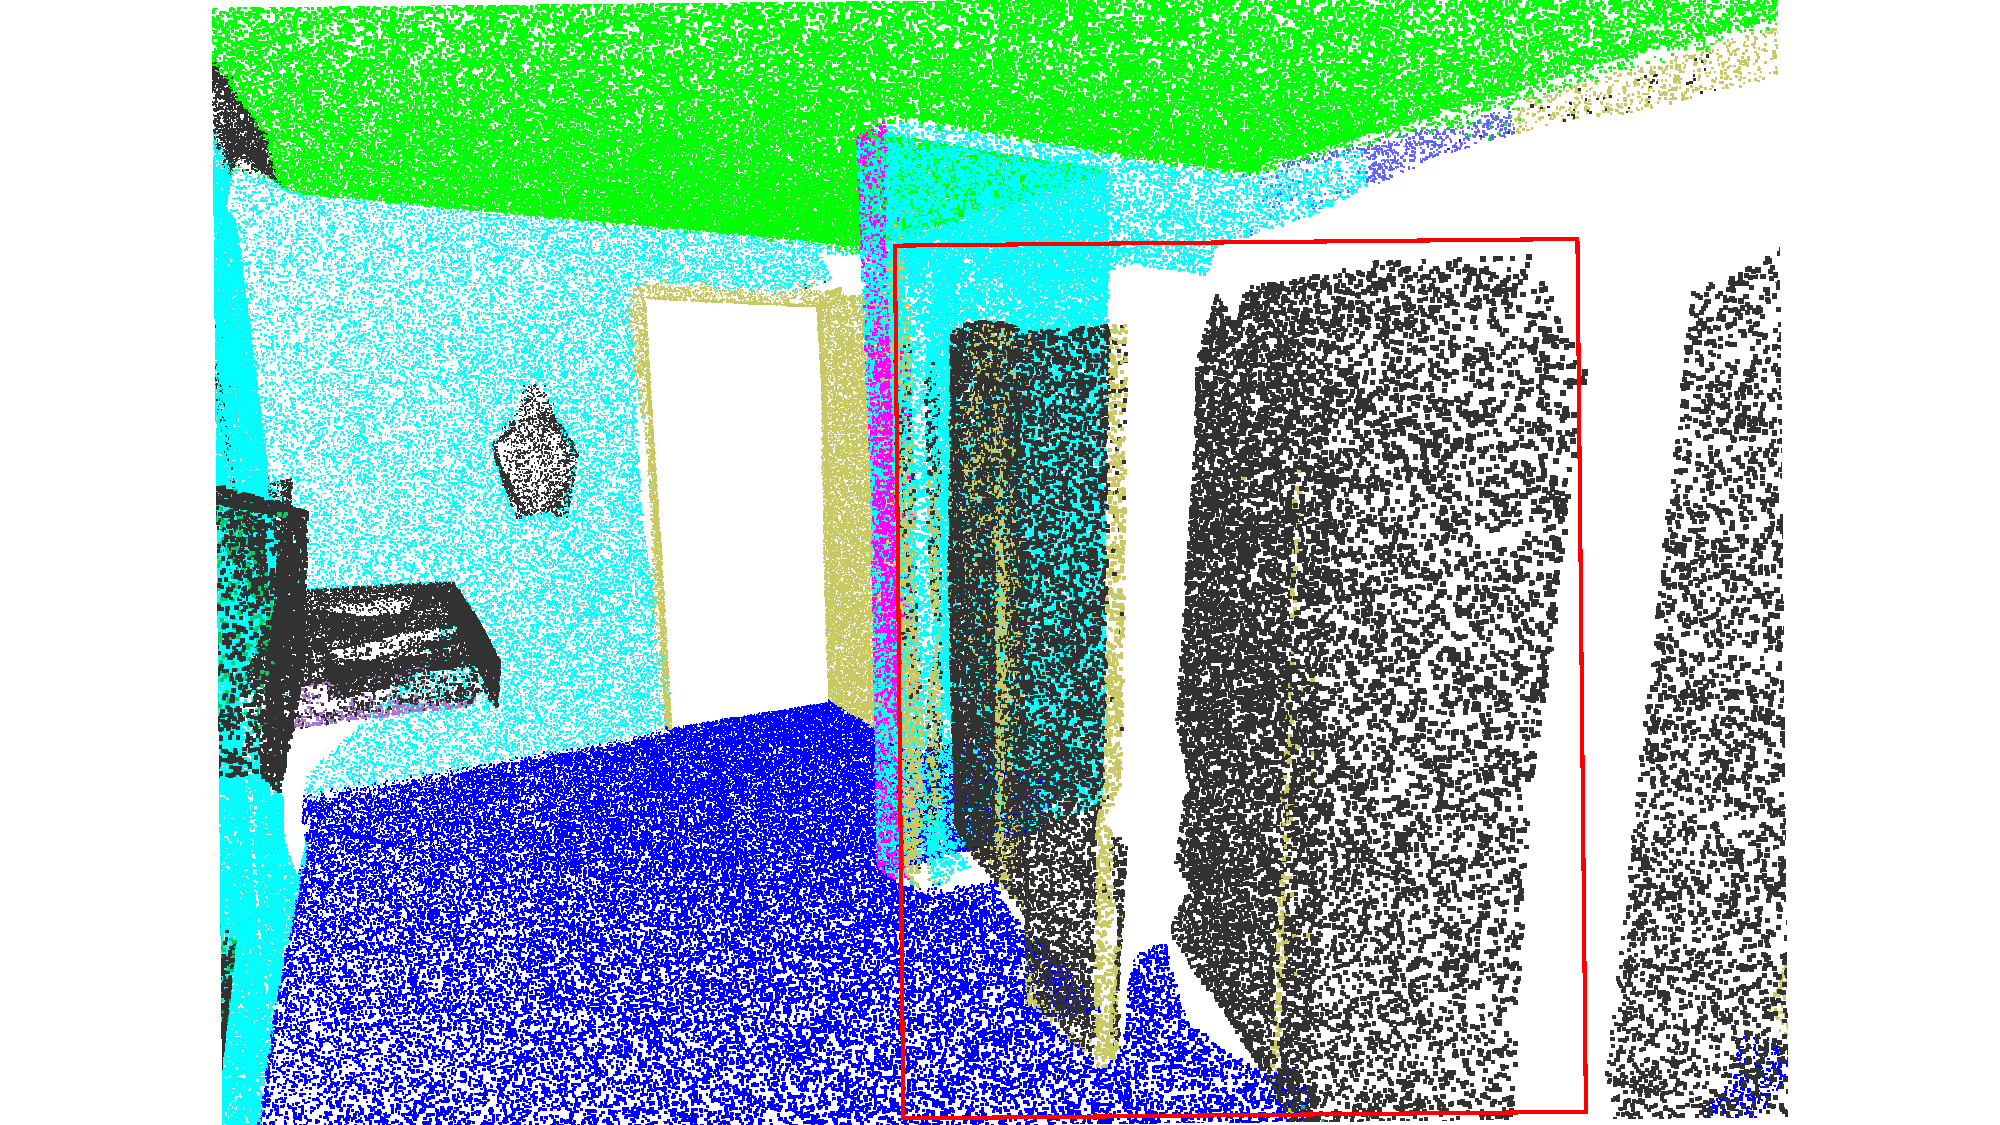
\includegraphics[width=\textwidth]{fig/supplement/semantic_segmentation/wc_2/PLT_wc_2.pdf}
    \end{minipage}
    \hfill

    % 换行
    \vspace{0.5em}

    % 第七行左侧的竖排标签
    \begin{minipage}{0.09\textwidth}
        \centering
        GT
    \end{minipage}
    \hfill
    % 第七行图片
    \begin{minipage}{0.22\textwidth}
        \centering
        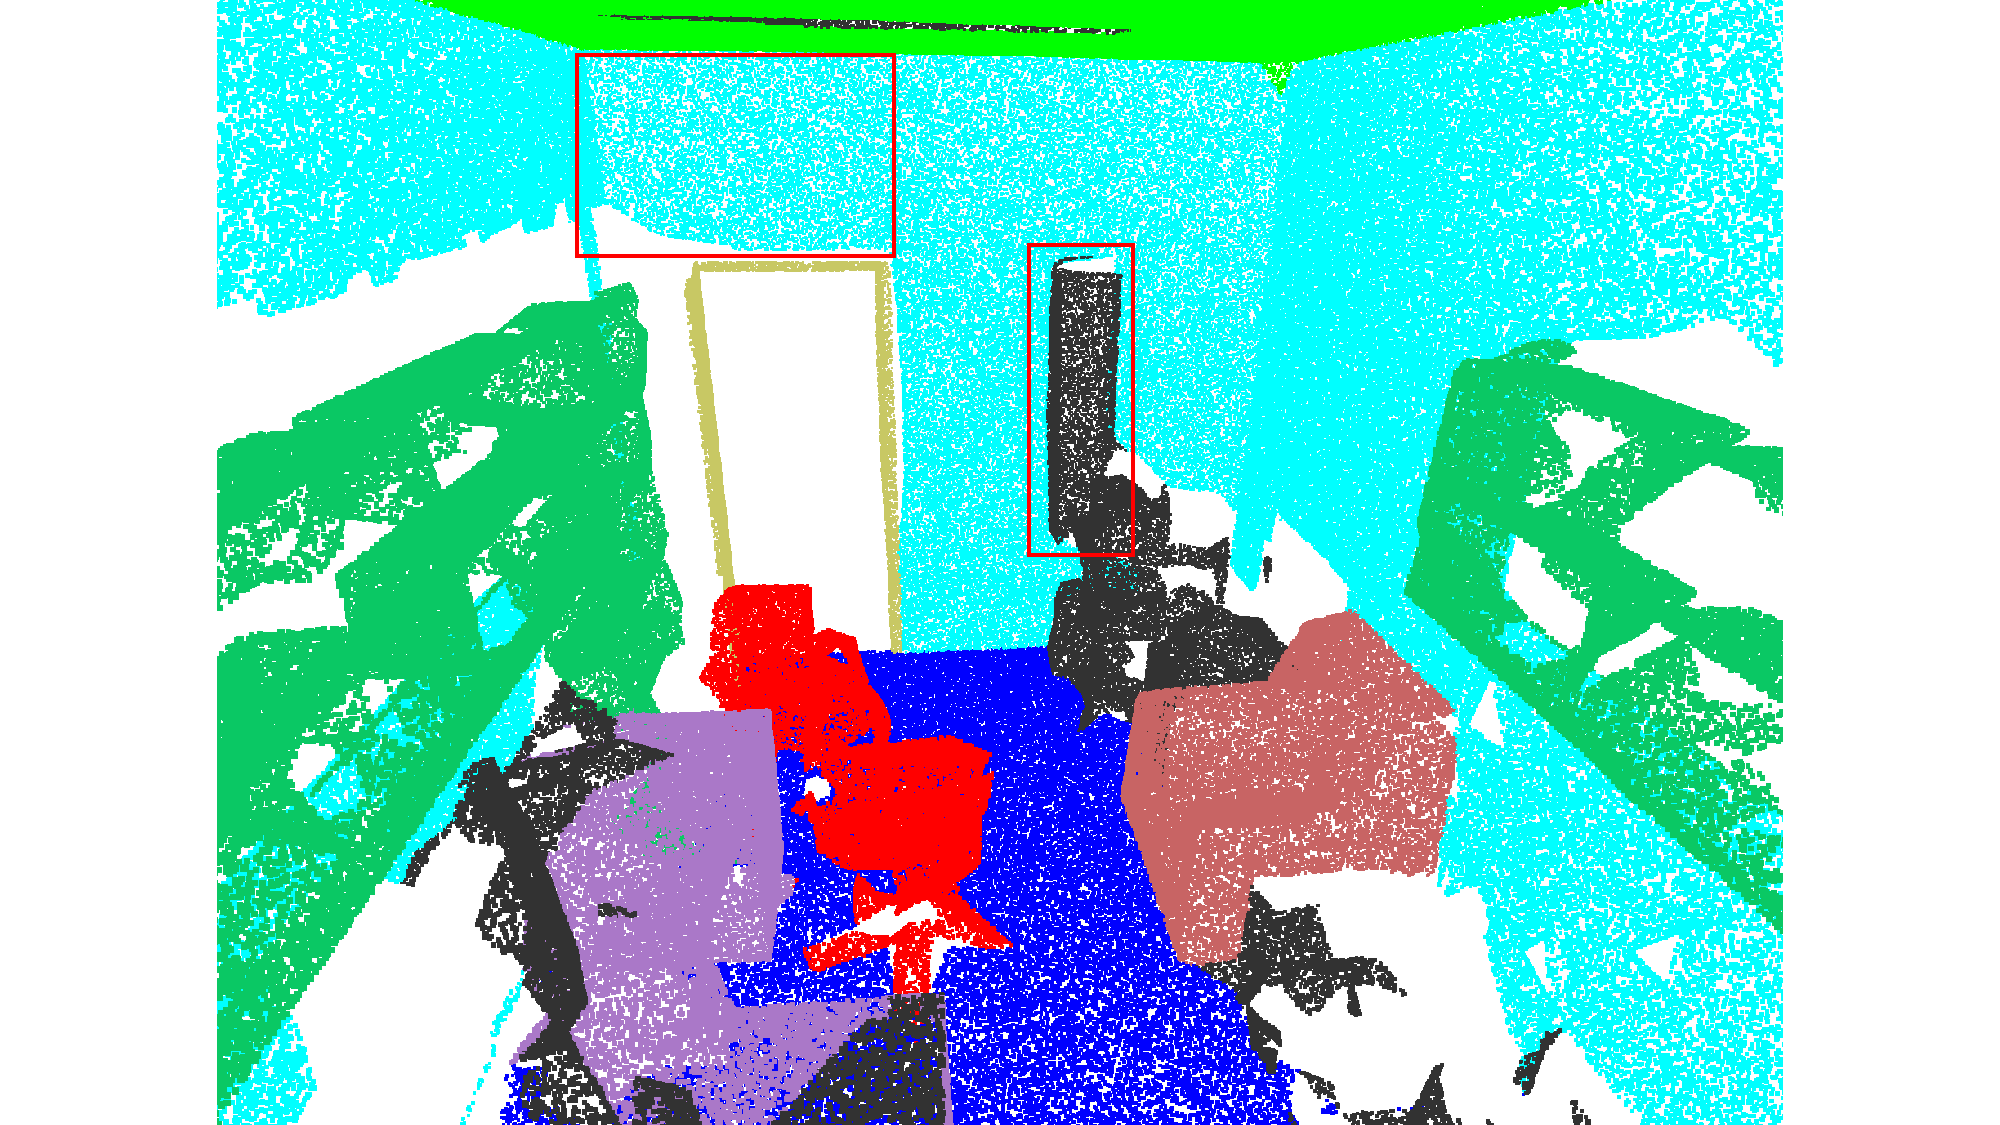
\includegraphics[width=\textwidth]{fig/supplement/semantic_segmentation/office_9/GT_office_9.pdf}
    \end{minipage}
    \hfill
    \begin{minipage}{0.22\textwidth}
        \centering
        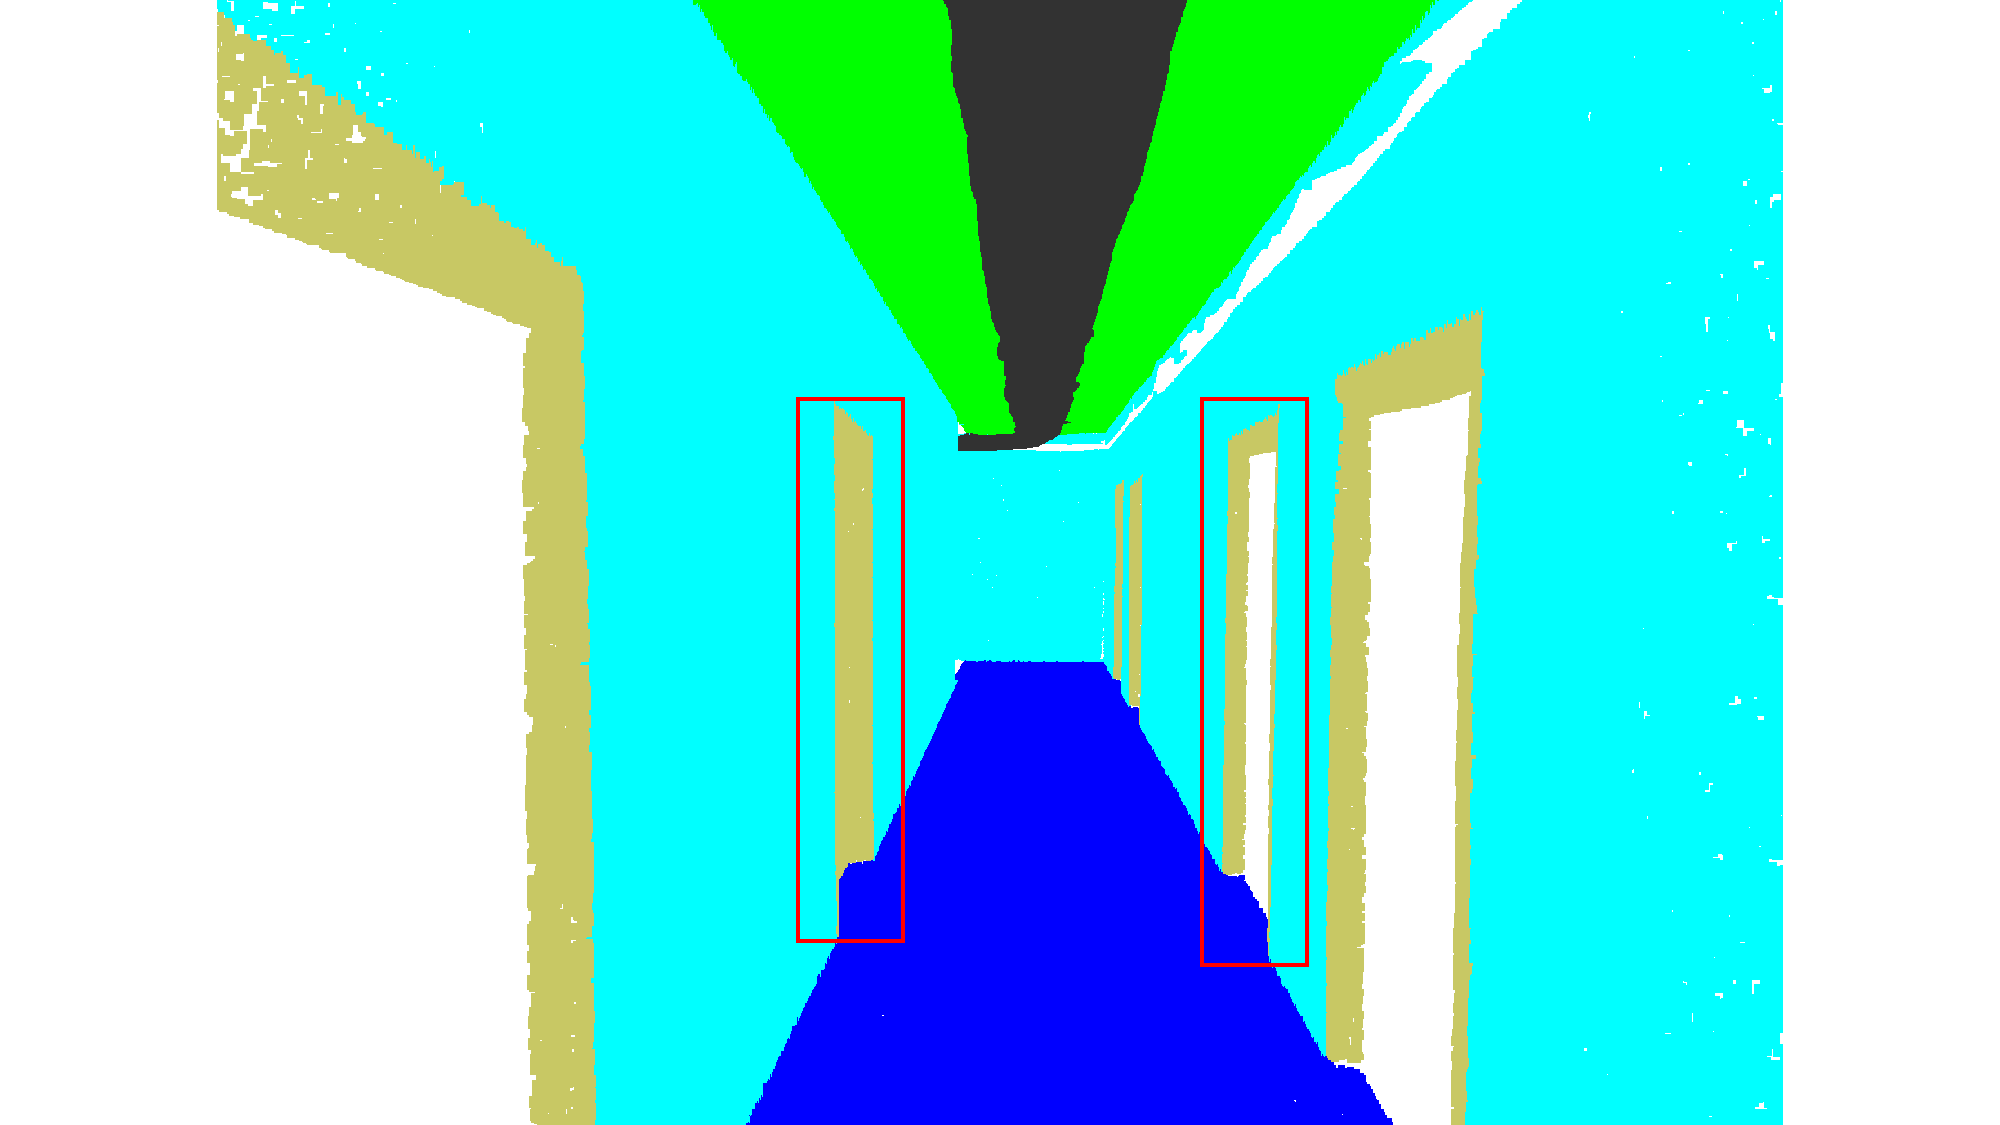
\includegraphics[width=\textwidth]{fig/supplement/semantic_segmentation/hallway_10/GT_hallway_10.pdf}
    \end{minipage}
    \hfill
    \begin{minipage}{0.22\textwidth}
        \centering
        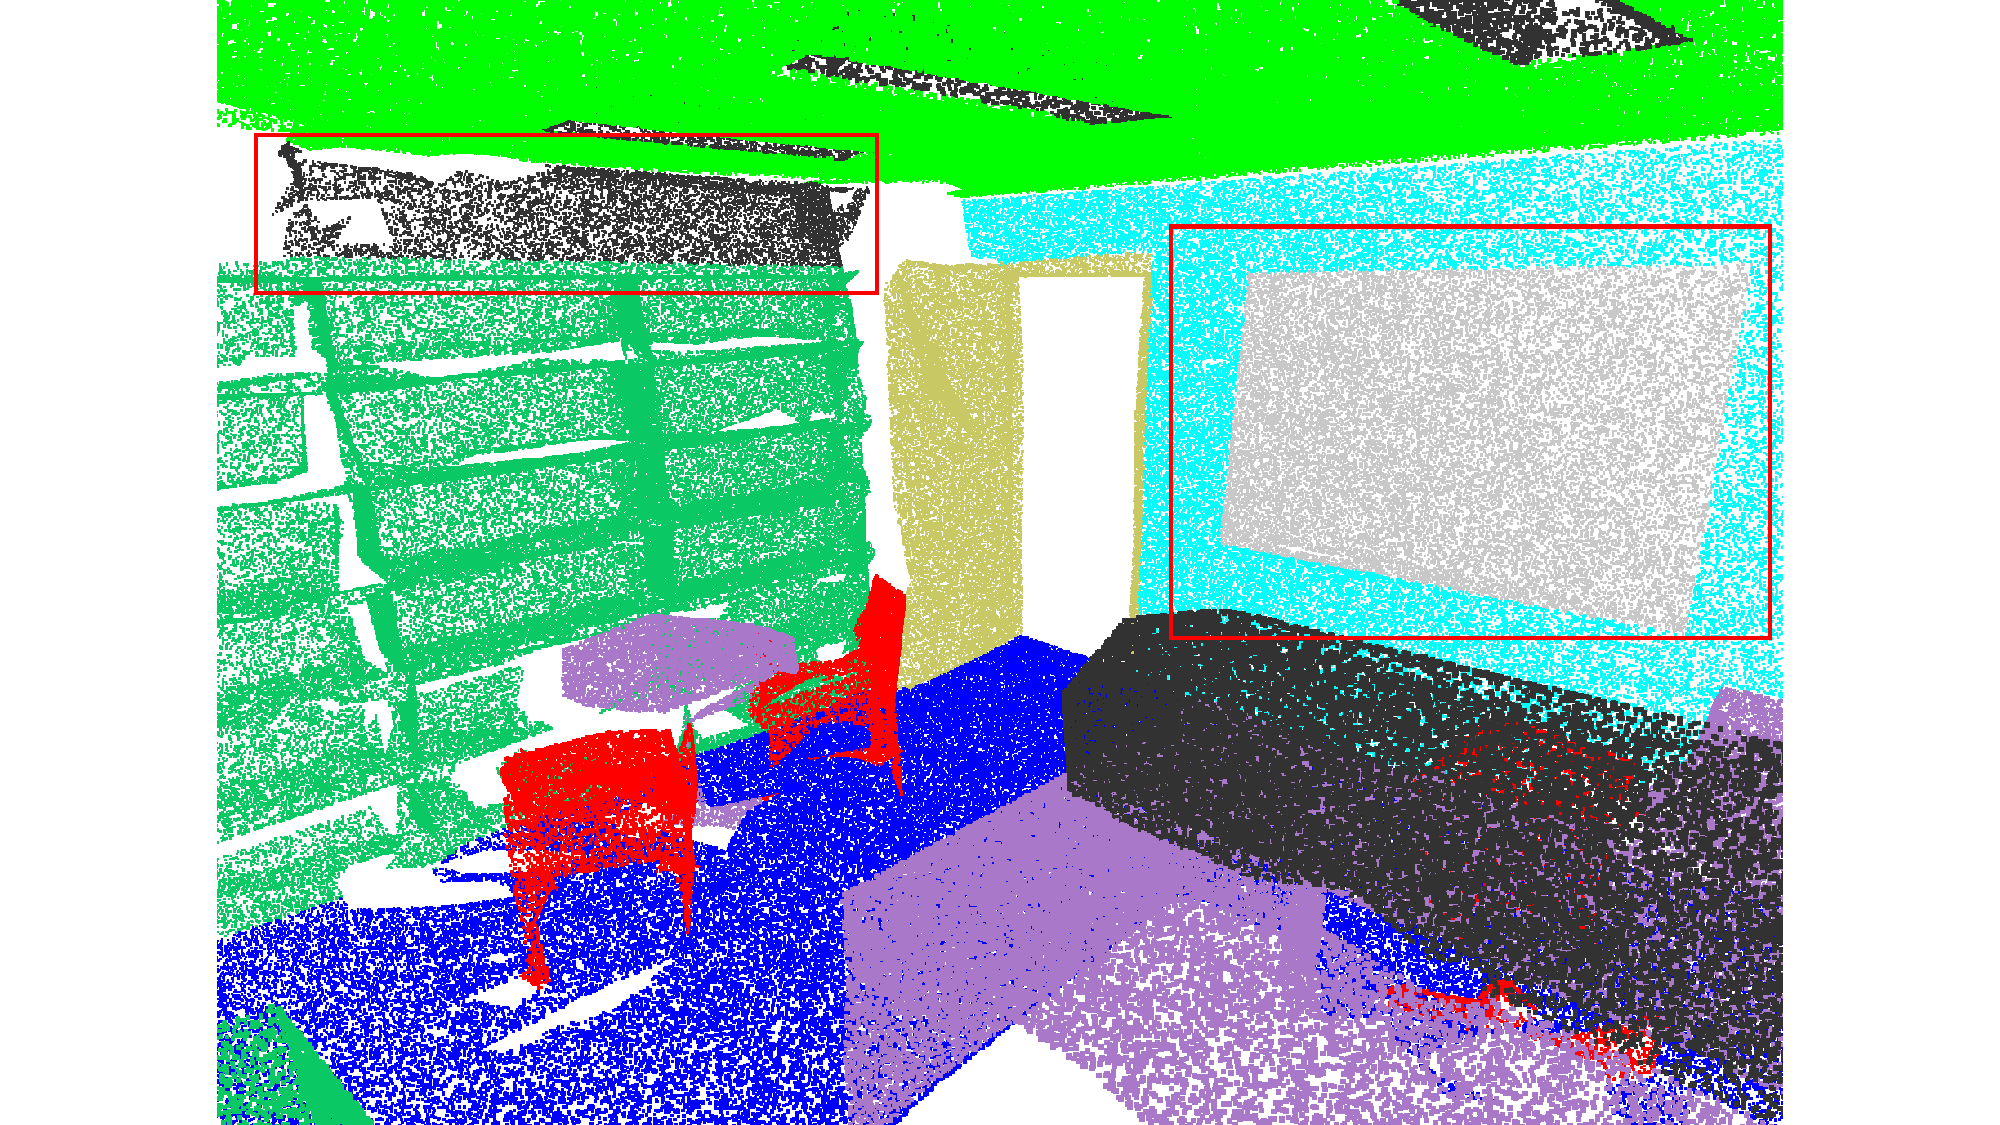
\includegraphics[width=\textwidth]{fig/supplement/semantic_segmentation/office_35/GT_office_35.pdf}
    \end{minipage}
    \hfill
    \begin{minipage}{0.22\textwidth}
        \centering
        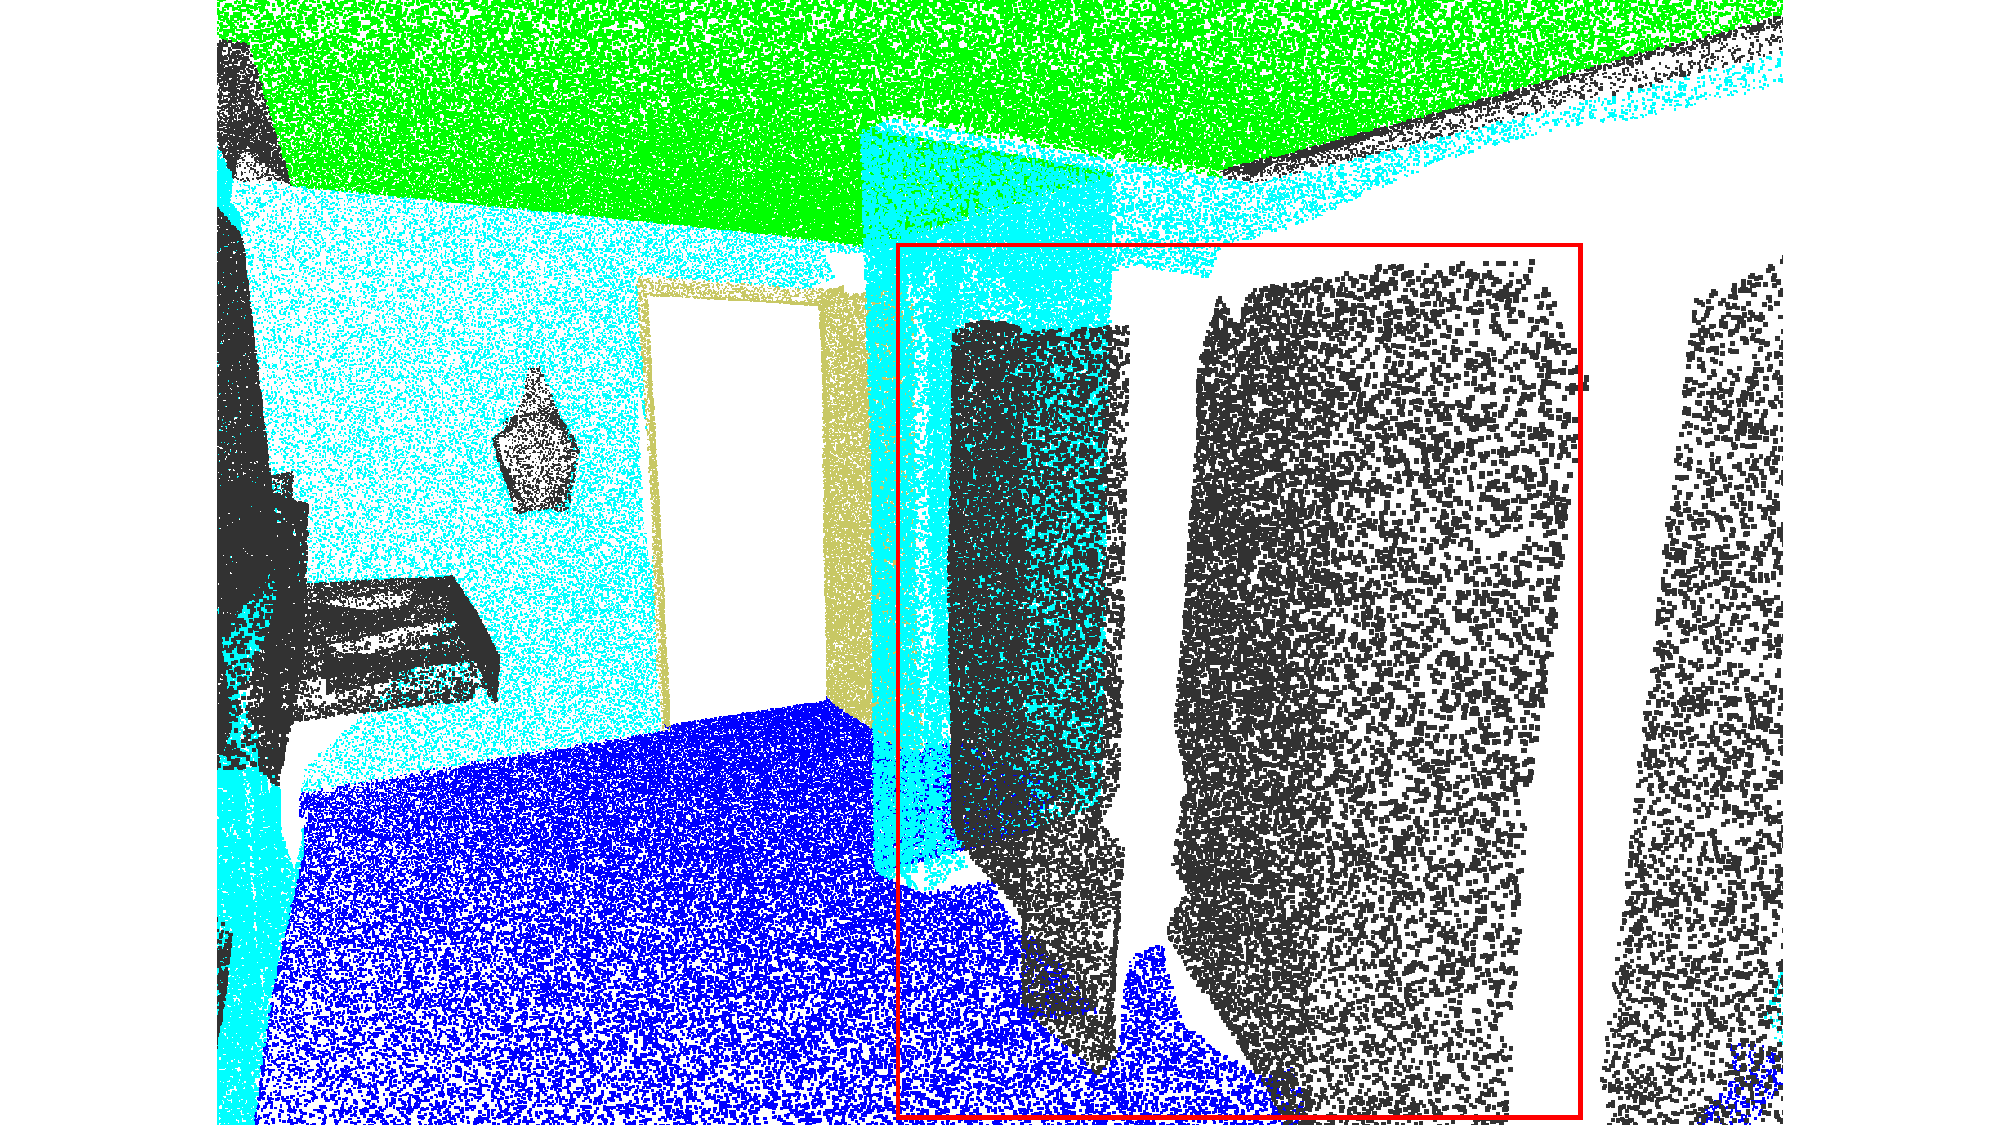
\includegraphics[width=\textwidth]{fig/supplement/semantic_segmentation/wc_2/GT_wc_2.pdf}
    \end{minipage}
    \hfill
    
    %下方的标签
    \vspace{0.5em}
    \begin{minipage}{0.09\textwidth} % 左侧空白区域
        \color{white}{12}
    \end{minipage}
    \hfill
    \begin{minipage}{0.22\textwidth} % 第2列标题
        \centering
        office\_9
    \end{minipage}
    \hfill
    \begin{minipage}{0.22\textwidth} % 第1列标题
        \centering
        hallway\_10
    \end{minipage}
    \hfill
    \begin{minipage}{0.22\textwidth} % 第3列标题
        \centering
        office\_35
    \end{minipage}
    \hfill
    \begin{minipage}{0.22\textwidth} % 第3列标题
        \centering
        wc\_2
    \end{minipage}
    \hfill
    \caption{The visualization of qualitative results for point cloud semantic segmentation. We compare our PLT with previous methods on Area 5 of the S3DIS dataset~\cite{armeni20163d}.}
    \label{fig:s3dis_1}

\end{figure*}
